%\documentclass[paper]{geophysics}
\documentclass[paper,revised]{geophysics}
\usepackage{cleveref} %for cref


% An example of defining macros
\newcommand{\rs}[1]{\mathstrut\mbox{\scriptsize\rm #1}}
\newcommand{\rr}[1]{\mbox{\rm #1}}
\usepackage{natbib}
\bibliographystyle{plainnat}
\begin{document}

\title{An example \emph{Geophysics} article, \\ with a two-line title}

\renewcommand{\thefootnote}{\fnsymbol{footnote}} 

\ms{GEO-Example} % paper number

\address{
\footnotemark[1]BP UTG, \\
200 Westlake Park Blvd, \\
Houston, TX, 77079 \\
\footnotemark[2]Bureau of Economic Geology, \\
John A. and Katherine G. Jackson School of Geosciences \\
The University of Texas at Austin \\
University Station, Box X \\
Austin, TX 78713-8924}
\author{Joe Dellinger\footnotemark[1] and Sergey Fomel\footnotemark[2]}

\footer{Paper}
\lefthead{Vikas \& Vikas}
\righthead{\emph{Geophysics}}

\maketitle

\begin{abstract}
  Seismic imaging remains a challenge for the oil and gas industry, even with advanced algorithms like Full Waveform Inversion (FWI). The effectiveness of FWI is highly sensitive to the initial model, which is typically constructed by conventional tomography models. Here, we propose a technique for preparing the initial model based on Particle Swarm Optimization (PSO), a global optimization method inspired by the social behavior of bird flocks. PSO utilizes the collective intelligence and movement patterns of birds to explore and optimize complex, multi-dimensional problem spaces, making it well-suited for refining initial models in seismic inversion tasks. Global optimization heuristic methods involve tuning parameters that affect both accuracy and convergence rates. In our implementation of PSO, we conducted experiments with well-defined nonlinear functions—Ackley, Griewank, Rastrigin, Styblinski-Tang, and Schwefel—to evaluate various parameter settings and determine those that achieve higher convergence rates. These optimized settings were then used in our inversion process to prepare the initial model. The number of model parameters involved in seismic inversion presents a significant challenge for global optimization methods due to the "curse of dimensionality," where the complexity of the optimization problem grows with the number of parameters. To mitigate this issue, we employed a simplified model defined by just three parameters: velocity at the interface, velocity gradient between interfaces, and depth of the interface. In this approach, we use prominent peaks in near-offset traces to invert a 1D depth velocity slice for multiple shots. These 1D velocity slices are then interpolated to form a 2D velocity model, which is smoothed before serving as the initial model for FWI. This method also addresses the computational time challenges associated with global optimization techniques. We validated the reliability of this technique using benchmark models designed to test inversion algorithms. Our results indicate that this method effectively prepares an initial model suitable for FWI. However, the technique is susceptible to errors in selecting the peaks from the seismic data.
\end{abstract}

\section{Introduction}

Full Waveform Inversion (FWI) is considered one of the most efficient seismic imaging methods due to its ability to utilize all seismic phases present in the data \citep{Pratt1999, Schuster2017, Tarantola1986, Virieux2009a}. This involves comparing synthetic data with observed data \citep{Gomez2017, Liu2017, Metivier2018}, where the difference between them is known as the objective function. The rate of change of the objective function with respect to model parameters \citep{Plessix2006} is used to iteratively update the model until the synthetic data from the updated model matches the observed data.
\par
The nonlinear relationship between synthetic data and model parameters \citep{Crase1990, Geng2018, Guo2021} leads to a multimodal nonlinear objective function, characterized by multiple local minima and maxima \citep{TenKroode2013}, as shown in \ref{fig:nonlinear_func}. FWI utilizes calculus-based optimization methods, such as gradient descent, BFGS, and conjugate gradient, which typically direct the solution towards the nearest extrema. This can lead to FWI becoming trapped in local minima if the starting model is not within the basin of attraction \citep{FitchnerETH2015}. Consequently, if the starting model is in a localized basin of attraction, achieving convergence to the global minimum becomes impossible. Therefore, it is crucial to initialize the inversion with a model that is close to the global minimum.
%\begin{figure}	
%	\centering
%	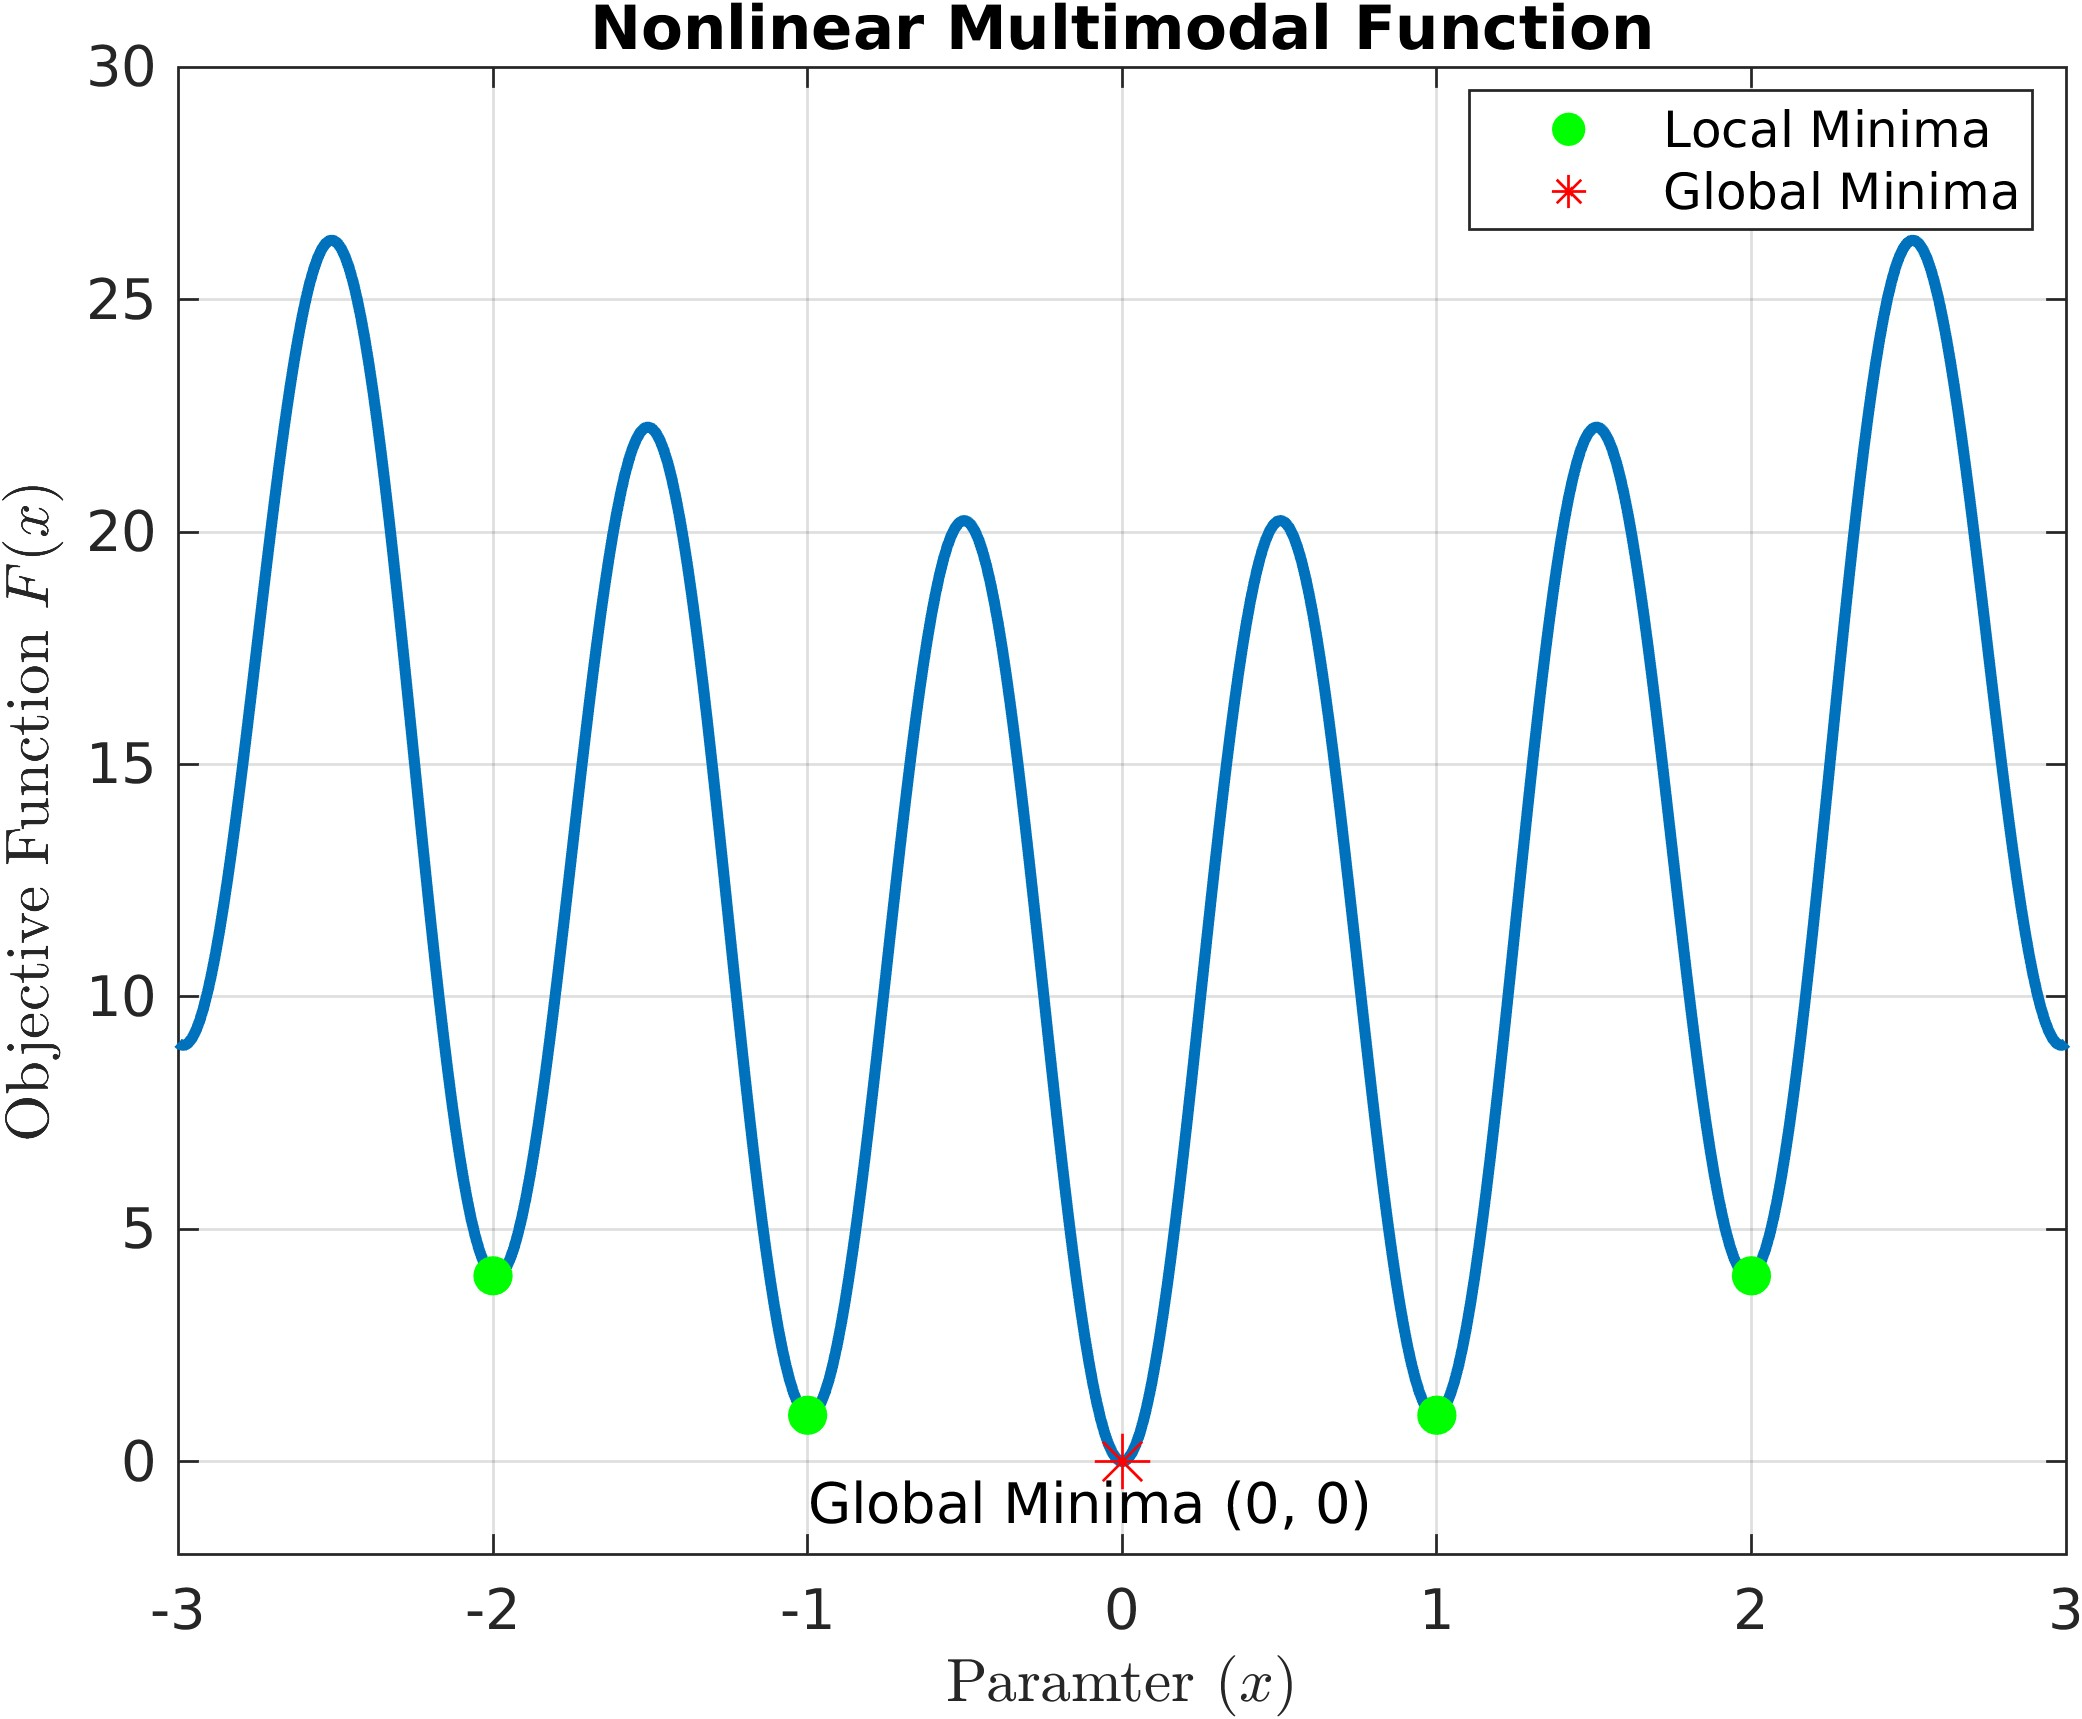
\includegraphics[width=0.5\paperwidth]{Fig/nonlinear_func.jpg}
%	\caption{Nonlinear multi-modal function.}
%	\label{fig:nonlinear_func}
%\end{figure} 
\par
FWI has undergone extensive research to address nonlinearity, focusing on both modifying the objective function and developing effective methods for preparing initial models through global optimization. Approaches to modifying the objective function include multiscale strategies \citep{Bunks1995a, Ravaut2004, Schafer2014, Sirgue2004}, which start with low-frequency data for initial inversions and gradually incorporate higher frequencies. The normalized cross-correlation objective function \citep{Chi2015, Liu2017} emphasizes phase matching to mitigate amplitude variations, while the envelope-based objective function \citep{Borisov2018, Chi2014} is used for updating long-wavelength models. More recent methods, such as the optimal transport function \citep{Brossier2016, Metivier2016, Metivier2018}, enhance the convexity of the basin of attraction, thereby increasing the likelihood that the initial model will fall within the basin of attraction for the global minimum.

In geophysics, common global optimization methods for preparing initial models in seismic inversion include Very Fast Simulated Annealing (VFSA), inspired by the annealing process in metallurgy \citep{Ingber1989, Kirkpatrick1983, Sacks1989}; Genetic Algorithm (GA), based on Darwin's theory of survival of the fittest \citep{Katoch2021, Michalewicz1996}; and Particle Swarm Optimization (PSO), which utilizes the concept of swarm intelligence \citep{Couceiro2016, Kennedy, Shi1999, Wang2018}. These methods, inspired by natural phenomena and expressed through mathematical formulations, are adept at exploring the entire search space to identify optimal solutions. The strategy involves a two-step process: initially using global optimization techniques to prepare the starting model, followed by FWI. This approach leverages the extensive exploration capabilities of global optimization methods \citep{Dong2015, Ye2024}. Once a reliable initial model is established, which is expected to be within the basin of the global minimum, local optimization methods are then applied due to their high exploitation efficiency.

Published implementations of these global optimization methods include a variety of approaches for geophysical data inversion. \cite{Datta2016} used VFSA for initial model preparation in a two-step process, employing zero-offset sections for parameterization. \cite{Fu2021} introduced a parallel VFSA algorithm for 1.5D acoustic FWI, allowing simultaneous updates of model parameters across multiple threads. \cite{Shiba2005} demonstrated VFSA's effectiveness in estimating earthquake displacement, showing its superiority over GA for this task. \cite{Mendes2024} utilized a training image to guide the generation of realistic velocity model samples, improving convergence. \cite{Datta2019} applied VFSA to represent sedimentary layers and salt bodies using interfaces and ellipses, respectively. On the GA front, \cite{Mazzotti2016} proposed a method with two grids—a coarse grid for inversion and a fine grid for modeling. \cite{Ktran2012} highlighted GA's potential for enhancing subsurface property characterization, while \cite{Zeng2011} explored GA for Rayleigh wave inversion. \cite{Aleardi2017} integrated GA with Markov Chain Monte Carlo (MCMC) methods to address search space uncertainties. In PSO applications, \cite{Yang2017} developed a PSO method for impedance inversion, \cite{Shaw2007} demonstrated its effectiveness in natural resource exploration, and \cite{Ding2015} focused on applying PSO to a 1D-DC resistivity case. Additionally, \cite{KaplanVural2020} showcased PSO's ability to invert common-offset ground-penetrating radar (GPR) traces and estimate dielectric properties, while \cite{Fernandez-Martinez2010} used PSO for reservoir characterization and \cite{Fern2010} explored its application to the SP inverse problem.
\par
A research also has been conducted to identify more effective global optimization methods. A comparison of Genetic Algorithms (GAs) with Monte Carlo methods found that GAs provide better fits with fewer model parameters and greater computational efficiency \citep{Sambridge1992}. Further analysis comparing GA with Particle Swarm Optimization (PSO) concluded that PSO generally outperforms GA \citep{Ding2015, Mojica2019}. Additionally, \cite{Sajeva2017} offers a comparative analysis of four stochastic optimization methods—adaptive simulated annealing (ASA), GA, neighborhood algorithm (NA), and PSO—for 1D elastic full-waveform inversion and residual static computation. The study indicates that the choice of optimization method should depend on the characteristics of the objective function and the dimensionality of the model space.
\par
In this study, we present the application of PSO for generating an initial model for FWI,due to its ability to effectively balance exploration and exploitation within the solution space. The implementation of global optimization methods in seismic inversion faces the challenge of the curse of dimensionality due to the large number of model parameters involved \citep{nirmit2024}. This necessitates defining the model with a reduced number of parameters. To address this, we have defined the model in terms of depth and velocity at the interfaces, as well as the rate of change of velocity between these interfaces. The number of interfaces to be inverted is determined solely by the selected number of breaks. The depth and number of interfaces are constrained by the arrival times of major breaks observed in near-offset seismic trace, respectively. Meanwhile, the velocity at each interface and the rate of change of velocity are limited by realistic subsurface velocity values. For near-offset receivers, these major breaks are most likely caused by reflections. This inversion begins with a uniform 1D velocity-depth model and sources positioned at various horizontal locations. Using this method, the interfaces are inverted progressively from the surface to depth. The data inverted for a particular interface serves as the initial model for the inversion of the subsequent interface. This process is repeated for all shots, with 1D velocity-depth profiles interpolated to prepare a 2D initial model for FWI. We also conducted experiments to find the optimal combination of parameters. A multi-threaded computation is also implemented to simultaneously invert data for multiple shots.
\\
\\
This paper is organized into the following sections:
\begin{itemize}
	\item Methodology: This section provides a detailed description of the Particle Swarm Optimization (PSO) algorithm, including experiments for selecting optimization parameters. It also covers the implementation of PSO, model parametrization, and offers a brief introduction to FWI.
	\item Results: This section presents the experiments conducted to prepare initial models for various benchmark seismic models to assess the reliability of the proposed method. It also includes the results of FWI applied to these initial models.
	\item Discussion and Conclusion: The section includes a discussion on the limitations of our method, its advantages over traditional techniques, and potential directions for future research.
\end{itemize}
\ref{method}
\section{Methodology}
This approach involves two steps. First, a coarse velocity model is prepared using PSO by optimizing the depth, interface velocity, and the rate of change of velocity between interfaces. This model serves as an initial model for conventional gradient-based FWI in the second step.
\subsection{Particle Swarm Optimization}
Particle Swarm Optimization (PSO) is a stochastic method developed by James Kennedy and Russell Eberhart in 1995. Inspired by the social behavior of birds flocking to find food, they formulated a mathematical model to simulate this behavior. This model is widely applied to solve various optimization problems. They identified that the fundamental principle guiding birds' food-finding behavior is their ability to communicate with each other. Each bird in the process knows its current position \((\mathbf{x}_i(t))\) and best position \((\mathbf{p}_i(t))\), determined by evaluating the fitness using a cost function. Additionally, each bird shares its best position with others, contributing to the collective knowledge of the flock's best position \((\mathbf{g}(t))\). Each bird's next movement is adjusted by its own best, the flock's best, and its current position. This iterative process continues at each step, ultimately converging towards a globally optimal position through the collaborative effort of all birds.This natural phenomenon is mathematically described by the velocity update equation \ref{eqn:pso_1} and the position update equation \ref{eqn:pso_2}.
\begin{itemize}
	\item \( \mathbf{x}_i(t) \) be the position of particle \( i \) at iteration \( t \).
	\item \( \mathbf{v}_i(t) \) be the velocity of particle \( i \) at iteration \( t \).
	\item \( \mathbf{p}_i(t) \) be the personal best position of particle \( i \) until iteration \( t \).
	\item \( \mathbf{g}(t) \) be the global best position among all particles until iteration \( t \).
	\item \( w \) be the inertia weight.
	\item \( c_1 \) and \( c_2 \) be the cognitive and social acceleration coefficients, respectively.
	\item \( r_1 \) and \( r_2 \) be random numbers uniformly distributed in the range \([0, 1]\).
\end{itemize}

The velocity and position update rules for each particle are given by:
\begin{equation}	
	\mathbf{v}_i(t+1) = w \mathbf{v}_i(t) + c_1 r_1 (\mathbf{p}_i(t) - \mathbf{x}_i(t)) + c_2 r_2 (\mathbf{g}(t) - \mathbf{x}_i(t))	
	\label{eqn:pso_1}
\end{equation}

\begin{equation}	
	\mathbf{x}_i(t+1) = \mathbf{x}_i(t) + \mathbf{v}_i(t+1)	
	\label{eqn:pso_2}
\end{equation}

Where:
\begin{itemize}
	\item \( w \) controls the influence of the previous velocity (inertia).
	\item \( c_1 \) and \( c_2 \) represent the trust of the particle in itself and in the swarm, respectively.
	\item \( r_1 \) and \( r_2 \) introduce stochasticity to the particle's movement.
\end{itemize}
\subsection{Optimization Parameters}
The updates in the Particle Swarm Optimization (PSO) algorithm are influenced by several controlling parameters, including the inertia weight \((w)\), acceleration coefficients \((c_1\) and \(c_2)\), population size of the swarm, and the number of iterations. Among these, the inertia weight is the most critical tuning parameter as it balances the exploration and exploitation capabilities of PSO by adjusting the contribution of the particle's previous velocity. An inertia weight value between 0.4 and 0.9 is generally found to provide good convergence. The cognitive and social coefficients \((c_1\) and \(c_2)\) represent the confidence in a particle's own best position and the swarm's best position, respectively, and they influence the updated velocity of the particles. The number of particles in the swarm also affects convergence; as the number of particles increases, the search space expands, potentially leading to better convergence. Experimental studies have shown that a swarm size of around 30 particles is generally effective for finding solutions within optimal iterations. The number of iterations, as with all iterative optimization algorithms, significantly impacts the performance of PSO.
\\
This contribution of different parameters for succes of PSO make it is necessary to decide the combination of these parameters precisely. we have performed experiments to find the optimal combination of this values, for these experiment we have choose four nonlinear multi-modal functions Ackley, Griewank, Rastrigin, and Styblinski-Tang function details of these functions are given in Appendix \cref{appendix_1} These experiments are performed to determine the optimal value of the optimization coefficient and examine the relationship between the number of iterations and swarm size. Since both swarm size and iteration count impact computational time, it is essential to balance these factors to achieve effective optimization while minimizing computational costs. To fairly compare the effects of swarm size and the number of iterations, the rate of increase for both parameters is kept consistent. Following, PSO is applied to the Schwefel function described in \ref{appendix_1} using the parameters selected from the previous experiment to identify those that yield optimal convergence. To analyze performance, accuracy is evaluated based on the maximum deviation using equation \ref{eqn:accuracy}. Further details of these experiments are outlined below.
\begin{equation}
	Accuracy (\%) = 100 - \left| \frac{optimal \ value - evaluated \ value}{optimal \ value - maximum \ deviation} \right| \times 100
	\label{eqn:accuracy}
\end{equation}
Where:
\begin{itemize}
	\item \(Optimal \  value\), best possible value of the objective function.
	\item \(Evaluated \ value\), value of the objective function at a given point in the feasible domain.
	\item \(Maximum \ deviation\), largest difference between the optimized value and the actual values.
\end{itemize}
\begin{enumerate}
	\item Accuracy with Parameters: In this experiment, optimization is conducted for all specified test functions using varying values of \(c_1\), \(c_2\), and inertia weights, as illustrated in figures \ref{fig:acc_ackley}, \ref{fig:acc_griewank}, \ref{fig:acc_rastrigin}, and \ref{fig:acc_styblinski}. To address the inherent randomness of this stochastic method, we perform 50 runs with 1000 iterations and calculate the average of these results as the final optimized values. 
	
This experiment concludes that a combination of inertia weights between 0.5 and 0.8, \(c_1\) values ranging from 0.6 to 2.0, and \(c_2\) values between 0.6 and 1.8 results in improved accuracy. 
%	\begin{sidewaysfigure}	
%		\includegraphics[width=\paperwidth]{Fig/ackley_para_vs_accuracy.jpeg}
%		\caption{Optimization of the Ackley function with varying inertia weights, \(c_1\), and \(c_2\) coefficients.}
%		\label{fig:acc_ackley}
%	\end{sidewaysfigure} 
%	\begin{sidewaysfigure}	
%		\includegraphics[width=\paperwidth]{Fig/griewank_para_vs_accuracy.jpeg}
%		\caption{Optimization of the Griewank function with varying inertia weights, \(c_1\), and \(c_2\) coefficients.}
%		\label{fig:acc_griewank}
%	\end{sidewaysfigure} 
%	\begin{sidewaysfigure}	
%		\includegraphics[width=\paperwidth]{Fig/rastrigin_para_vs_accuracy.jpeg}
%		\caption{Optimization of the Rastrigin function with varying inertia weights, \(c_1\), and \(c_2\) coefficients.}
%		\label{fig:acc_rastrigin}
%	\end{sidewaysfigure} 
%	\begin{sidewaysfigure}	
%		\includegraphics[width=\paperwidth]{Fig/styblinski_para_vs_accuracy.jpeg}
%		\caption{Optimization of the Styblinski-Tang function with varying inertia weights, \(c_1\), and \(c_2\) coefficients.}
%		\label{fig:acc_styblinski}
%	\end{sidewaysfigure} 

	\item Accuracy with iterations: Here, accuracy is assessed while maintaining a constant swarm size of 30 and an initial iteration count of 1000, which is then increased by factors of 1.67, 2.0, 2.67, 3.00, 5, and 10, to examine how the number of iterations impacts accuracy across all test functions. The results indicate that as the number of iterations increases, accuracy improves, reaching a maximum close to 100 \% when iterations are increased to 10 times, as illustrated in figure \ref{fig:acc_itr}.
%	\begin{figure}	
%		\centering
%		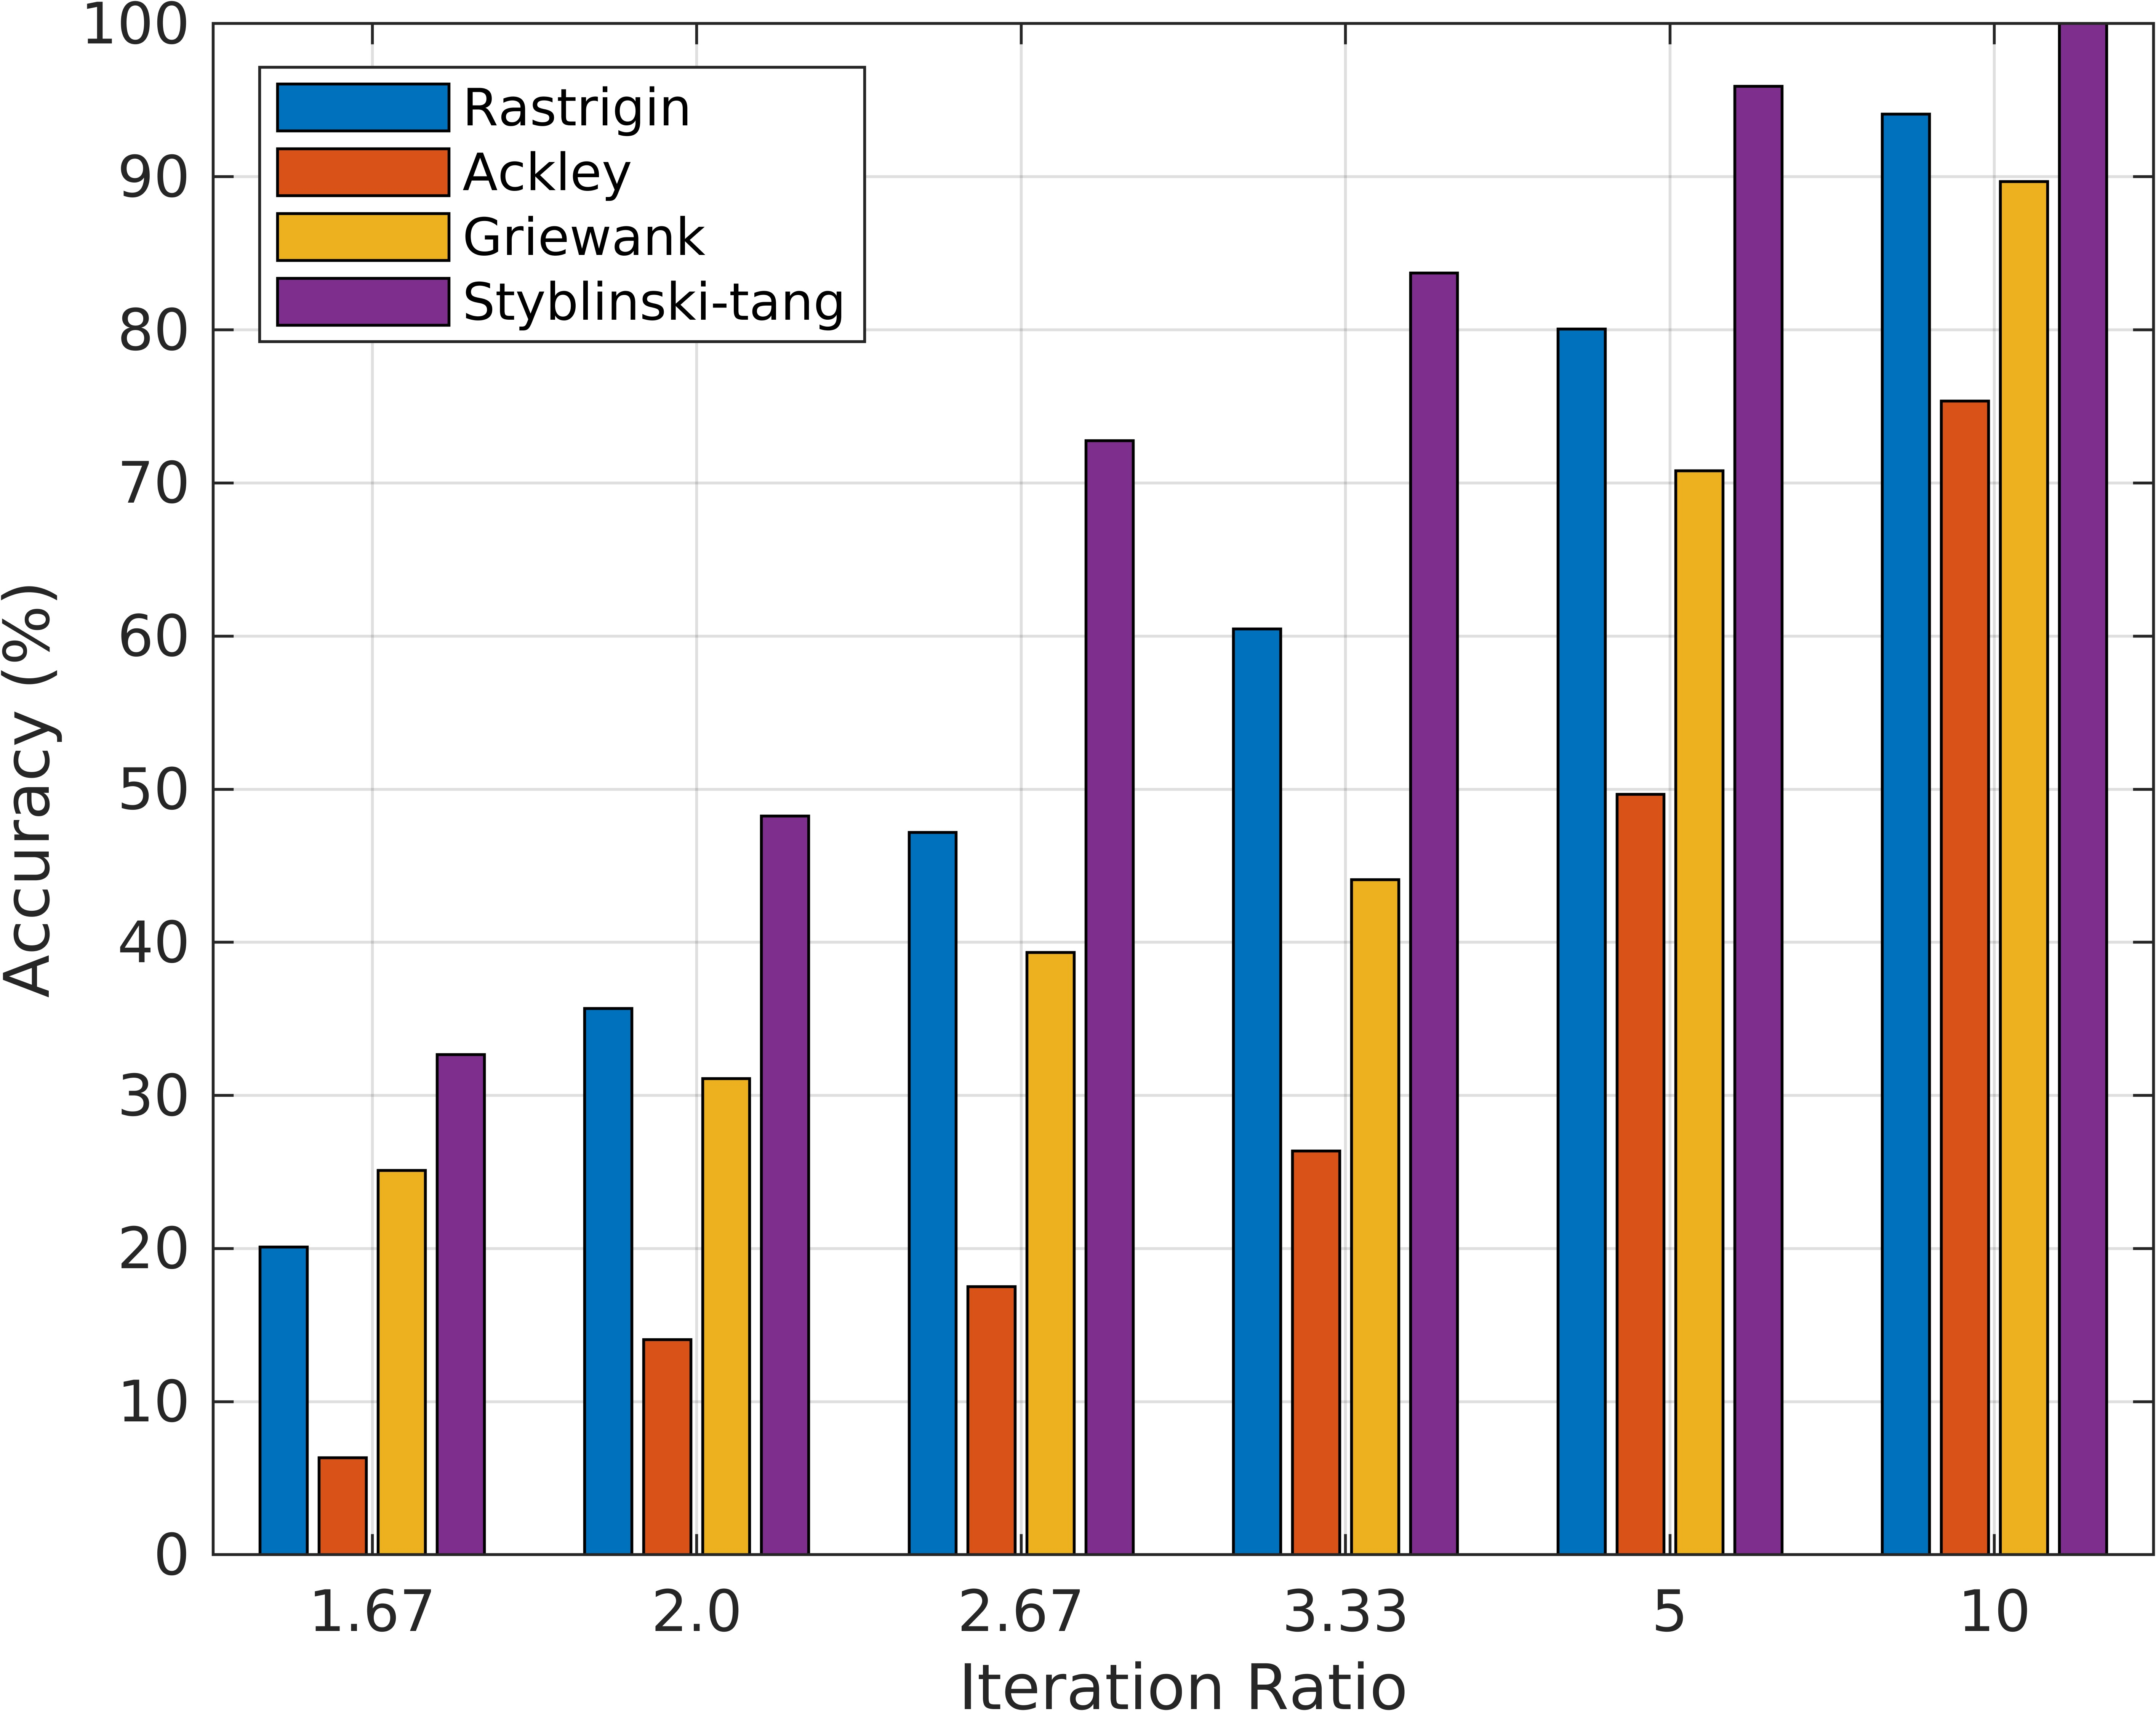
\includegraphics[width=0.7\paperwidth]{Fig/iteration_vs_accuracy.jpeg}
%		\caption{Accuracy variation with iterations keeping the swarm size at 30 for all test functions.}
%		\label{fig:acc_itr}
%	\end{figure}
	
	\item Acuuracy with swarm size: In this study, accuracy is evaluated across all tests by varying the swarm size, starting with 30 particles and increasing it by factors of 1.67, 2.0, 2.67, 3.00, 5, and 10, while keeping the number of iterations constant at 1000. The findings indicate that as the swarm size increases, accuracy improves to approximately 70 \%.
\end{enumerate}
From these experiments for finding the optimization parameters, it is concluded that an optimal combination of inertia weights between 0.5 and 0.8, \(c_1\) values ranging from 0.6 to 2.0, and \(c_2\) values between 0.6 and 1.8 leads to enhanced accuracy. Additionally, increasing the number of iterations relative to the number of particles is beneficial, as it provide improved accuracy while maintaining similar computational costs.
\\
The parameters that performed well in the previous experiments with test functions are used to evaluate the rate of convergence for the Schwefel function, as shown in Figure \ref{fig:schwefel}. This additional test function focuses solely on the objective function with respect to the number of iterations, as illustrated in figure \ref{fig:con_schwefel}. The aim of this study is to identify a combination of optimization parameters that achieve a better rate of convergence, enabling optimized results to be obtained within fewer iterations. Figure \ref{fig:con_schwefel} illustrates that higher values of inertia do not show convergence, while lower values of inertia exhibit a high rate of convergence but fail to reach the optimized value. An inertia value of 0.6 demonstrates good convergence with different \(c_1\) and \(c_2\) values. This analysis reveals that \(c_1\) at 1.8 and \(c_2\) at both 1.8 and 2.4 converge to zero, albeit slowly. In contrast, \(c_1\) at 2.4 and \(c_2\) ranging from 1.2 to 1.8 exhibit a good rate of convergence, reaching near zero within 100 iterations. Based on this analysis, the optimal parameters for further seismic inversion are set as inertia at 0.6, \(c_1\) at 2.4, and \(c_2\) between 1.2 and 1.8.

%\begin{figure}	
%	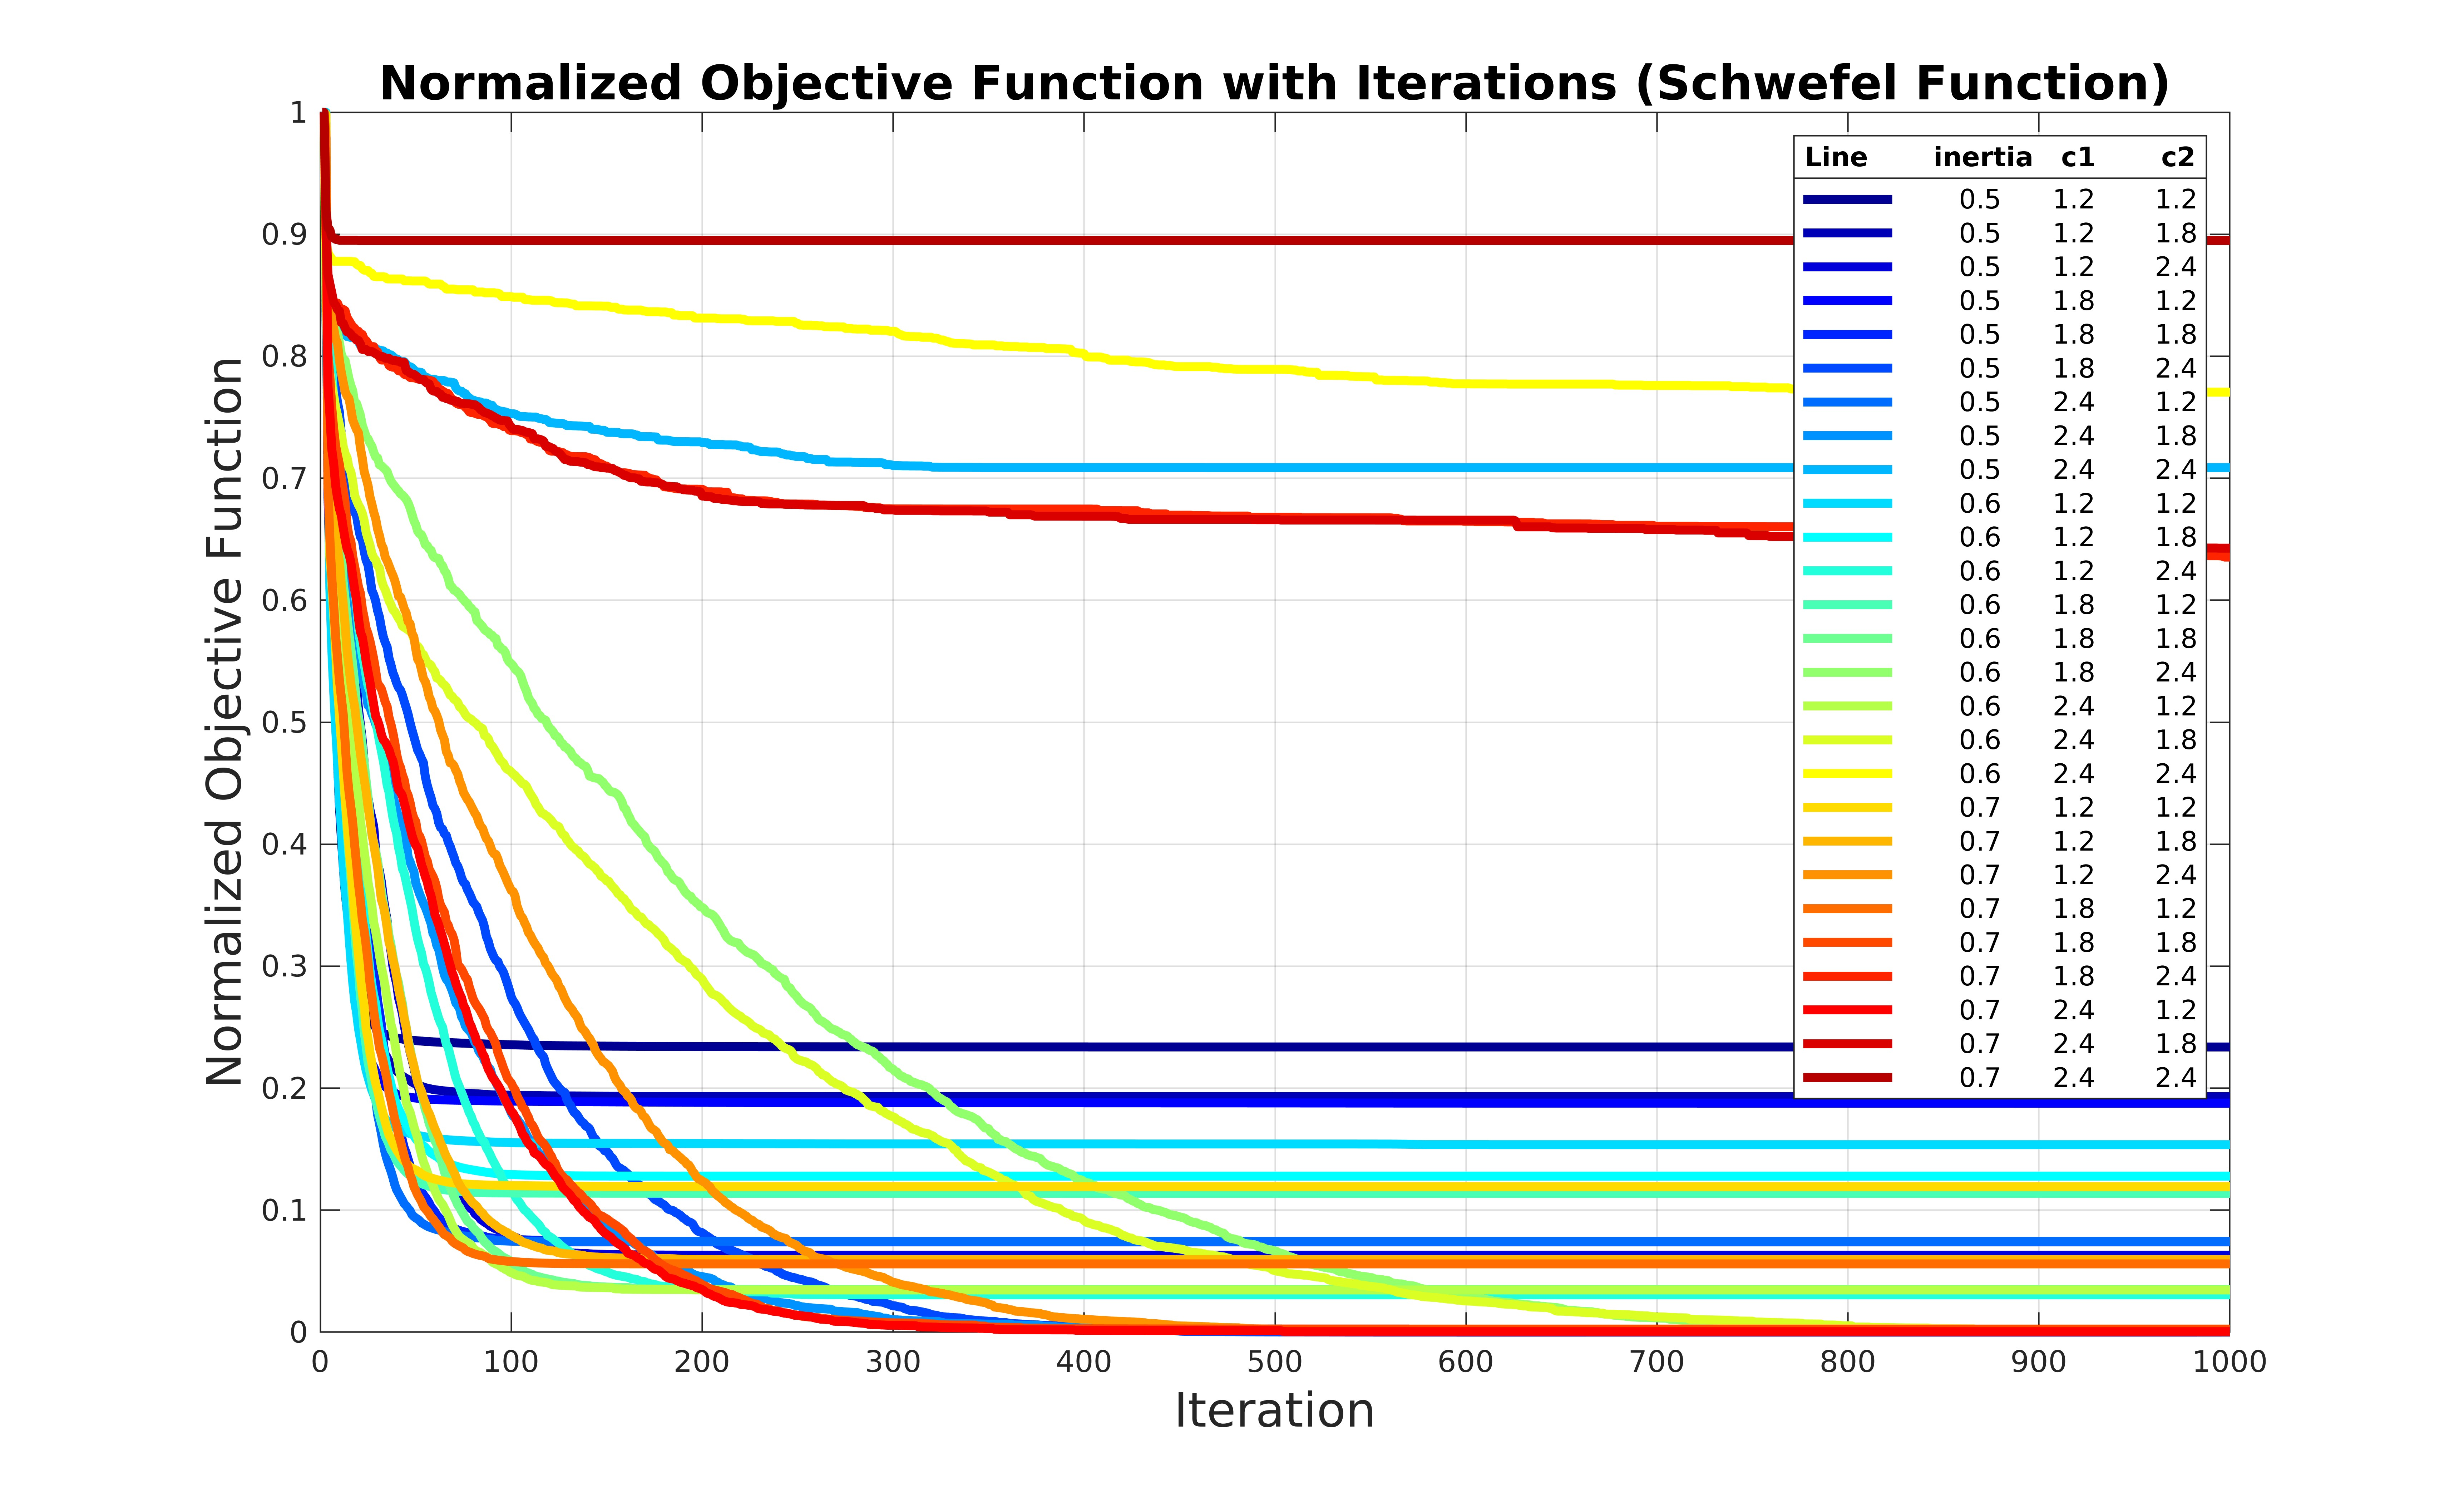
\includegraphics[width=0.8\paperwidth]{Fig/con_vs_itr.jpg}
%	\caption{Objective function versus iteration for Schwefel function.}
%	\label{fig:con_schwefel}
%\end{figure}

\subsection{Model Parameterization}
The seismic model includes physical parameters defined at densely packed grid points, often in the thousands, leading to an exponentially expanding search space that complicates the implementation of PSO. Therefore, it is essential to create a method for defining these velocity models with fewer parameters before implementing PSO, ensuring that the resulting output model can effectively serve as an initial model for FWI. 
\\
We propose a technique to define model with 1D depth-velocity profiles at sparse horizontal positions, as illustrated in Figure \ref{fig:parameterization} with white vertical lines. This model is representing a layered marine environment, where the velocity gradually increases with depth, ranging from 1500 to 4700 m/s. Additionally, it features a low-velocity layer situated between two high-velocity layers. The depth of interface in terms of grid point (\(d_i^k\)), where \(i\) represents the \(i^{th}\) interface for the \(k^{th}\) depth-velocity profile, (\(g_i^k\)) denotes the rate of change of velocity between the \((i - 1)^{th}\) and \(i^{th}\) interfaces, and (\(v_i^k\)) indicates the velocity of the model at the \(i^{th}\) interface.  These multiple, sparsely located depth-velocity profiles are interpolated using cubic splines to create an initial model. It is also assumed that no two interfaces intersect, as this is geologically implausible. Furthermore, the search space is restricted to feasible physical parameters. With these constraints, PSO is employed to optimize the three parameters for each layer in the development of the initial model.

%\begin{figure}	
%	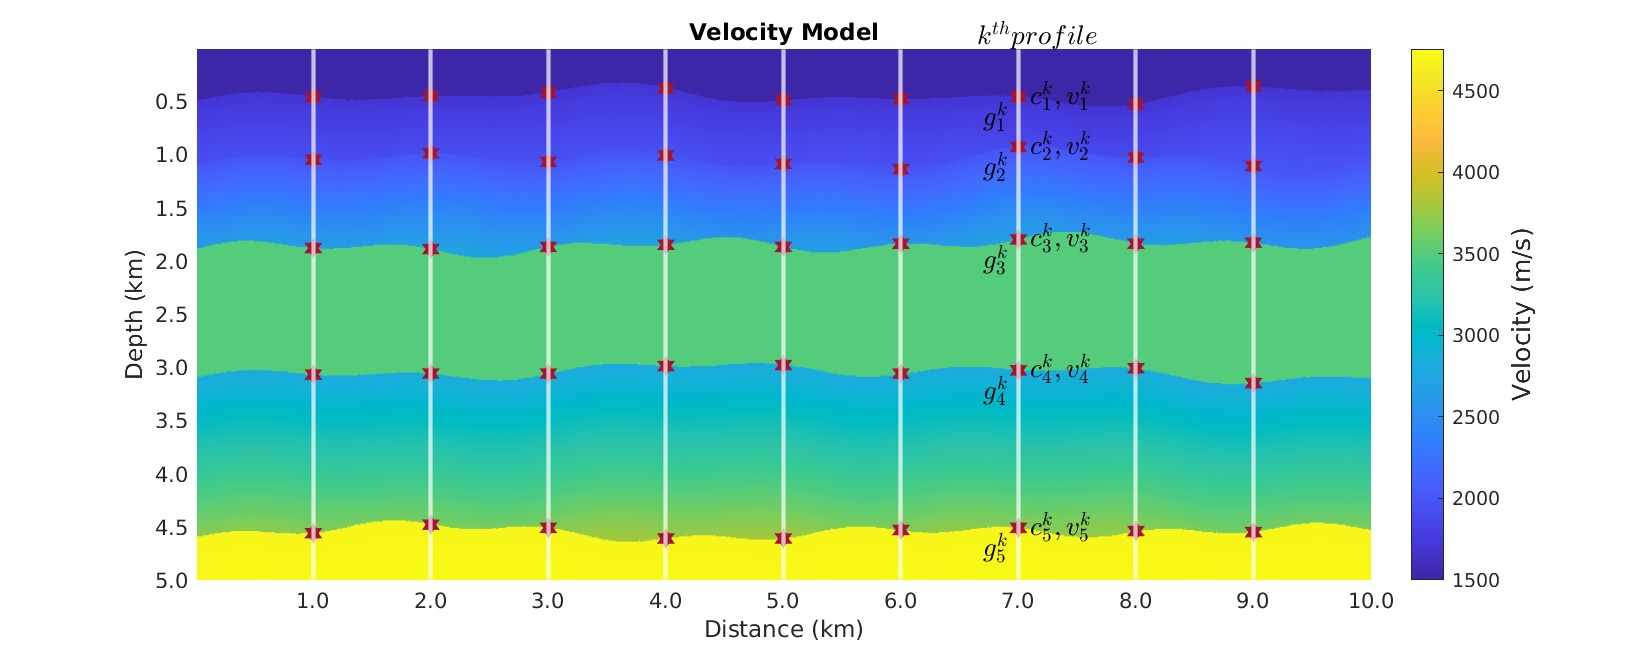
\includegraphics[width=0.8\paperwidth]{Fig/parameterization.jpg}
%	\caption{layered model.}
%	\label{fig:parameterization}
%\end{figure}

\subsection{PSO for Preparing Initial Model}
The workflow of this implementation is illustrated in Figure \ref{fig:work_flow}. It shows that initial model preparation begins with a uniform 1D depth-velocity profile as the initial model, where the velocity is same as upper layer and three parameters—depth, velocity at the interface, and the rate of change of velocity—are used as input parameters initially which are set to zero. A synthetic trace for this model is generated using an \(8^{th}\)-order spatial scheme and a \(2^{nd}\)-order temporal scheme. The synthetic trace is then compared to the observed data using the L2 norm, as described by equation \ref{eqn:l2norm}. The observed data consists only near-offset data, where the major peaks are likely caused by reflectors directly beneath the shot location. The major peaks are selected from the observed data to guide the inversion process, with a focus on progressively inverting the reflectors defined by grid points. This approach falls into the category of over-parameterization as explained by (Sen Stoffa 1991), where the model is described by microlayers with thickness equal to the grid spacing. The inverted model justifying a particular peak used as an initial model for the next one. This process is repeated until the inversion successfully accounts for all the selected peaks for a shot. We allow flexibility in the timing of the selected peaks since it is not always precise to pinpoint the exact peak. The peaks resulting from multiples will not significantly impact the model because the interfaces causing these multiples have already been accounted.
We sparsely select the shot locations and repeat this process for all chosen shots. Using the inverted reflectors from these shots, we create an initial model through interpolation and smoothing. This serves as the initial model for FWI.

%\begin{figure}	
%	\centering
%	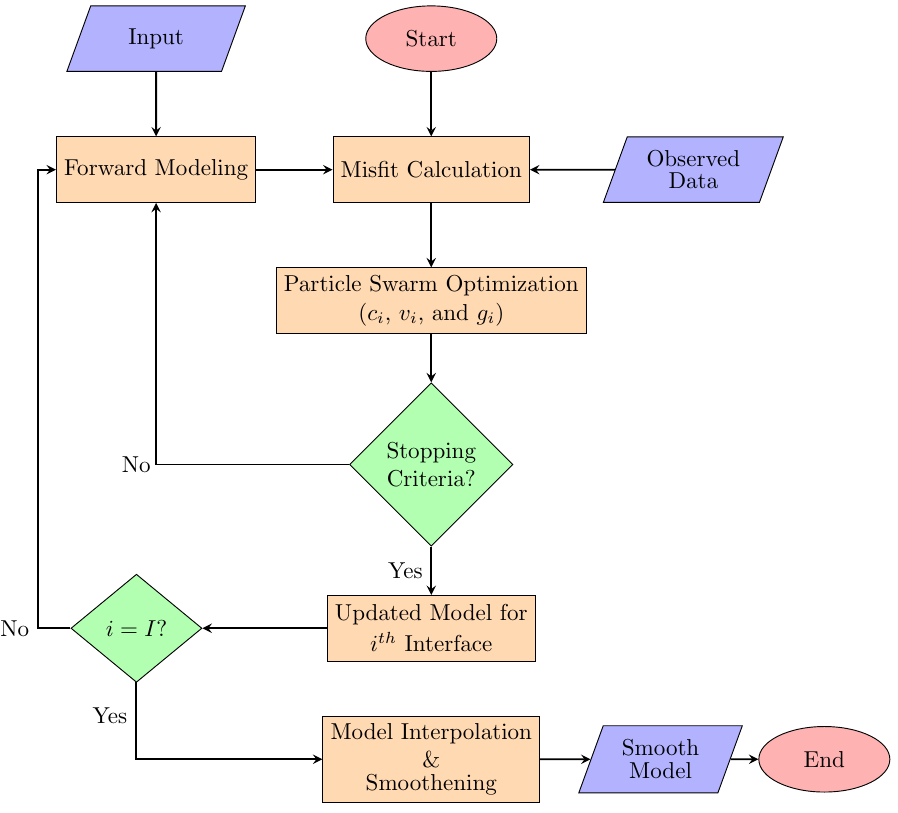
\includegraphics[width=0.5\paperwidth]{Fig/flow_chart.png}
%	\caption{Work-flow.}
%	\label{fig:work_flow}
%\end{figure}

\begin{equation}
	O(syn^k, obs^k) = \sqrt{\sum_{i=1}^{N} \left( syn^k - obs^k \right)^2}
	\label{eqn:l2norm}
\end{equation}

Where \(obs^k\) and \(syn^k\) indicate the observed data and synthetic data generated from the model, respectively; \(k\) refers to the shot number, and \(N\) represents the total samples.

\subsection{Full Waveform Inversion}
The model prepared using PSO serves as an initial model for FWI. Synthetic data is generated with this model and compared with the observed data, a process known as misfit calculation. Common methods for this calculation include the L2 norm, normalized cross-correlation function, Huber norm, and optimal transport function. The gradient of the objective function with respect to the model parameters is then calculated, which aids in updating the model. This iterative process ultimately leads to the recovery of velocity model.
\label{method}

\section{Results}
this proposed method is tested on benchmark models  X, Y, and Z these model have different complexity in structure and geological settings. intial model for these models is for implimentation of FWI is computed with our technique.  for preparing the initial model, 1D velocity depth slices for sparsely located shots at regular interval is selected for inversion of the near offset data. The initial velocity of the model used by global optimization is uniform and same as the velocity of the upper layer which is water for marine enviornment. Synthetic field for these model is prepared by numerically solving the acoustic wave equation with the finitie difference scheme, the source signautre is of 10 Hz frequency where the grid size is 10 m with temopral discretization of 1 ms. then FWI in time domain is performed using Shavi-1.0 (ref). a multiscale strategy is used in FWi where the inversion is started from a low frequncy whihc grdually increaed to recover the fine structure of model.
\\
parameter selection for intial model
\subsection{X}
\begin{itemize}
	\item model description
	\item model dimension
	\item discretization
	\item source and receiver information
	\item source and reciver selection for initla model preparation
	\item explain the initial model prepared
	\item FWi implementation
	\item explain 1D slice
	\item explain the seismogram
\end{itemize}
\subsection{Y}
\subsection{Z}
\section{Discussion}
\section{Conclusion}
we present a new approach of implimentation of PSO for preparing an initial model for FWI. In this technique, the employed parametrization technique sucessfuly define  the model this also reduce the  number of parameters involves in the inversion, subsequently reduce the complexity associated with the number of parameters to be inverted. For preparing the initial model near offset data for sparsely choosen shots are inverted to prepare a 1D depth velocity slices. this 1D slice address the challenges associated with computational cost of numerical modeling of seismic wave. 
we also show the reliablity of this technique by implimenting it on benchmark models. For all models sparsely located shots are selected for 1D inverting the near offset data.
\begin{itemize}
	\item 
\end{itemize}
\begin{acknowledgments}

\end{acknowledgments}

\append{Nonlinear Multimodal Functions} \label{appendix_1}
The Ackley, Griewank, Rastrigin, Styblinski-Tang, and Schwefel functions, illustrated in Figures \ref{fig:ackley}, \ref{fig:griewank}, \ref{fig:rastrigin}, \ref{fig:styblinski}, and \ref{fig:schwefel} respectively, are nonlinear multi-modal functions. These functions are commonly used to assess the performance of optimization algorithms due to their large number of local minima and nearly flat regions near the global minima. As the number of variables increases, the complexity of these functions also grows significantly, and their intricate topographies further complicate the search for solutions. This combination of features presents substantial challenges, making these functions ideal for testing optimization methods.
Their mathematical expressions are provided in Equations \ref{eqn:ackley}, \ref{eqn:griewank}, \ref{eqn:rastrigin}, \ref{eqn:styblinski}, and \ref{eqn:schwefel}.

{\bf{Ackley Function}}
\begin{equation}
	f(x) = -a \exp\left(-b \sqrt{\frac{1}{n} \sum_{i=1}^{n} x_i^2}\right) - \exp\left(\frac{1}{n} \sum_{i=1}^{n} \cos(c x_i)\right) + a + \exp(1)
\end{equation}
where \( a = 20 \), \( b = 0.2 \), and \( c = 2\pi \).\\
Global Minimum: \(f(x)=0\)\\
Location: \(x=0\)

{\bf{Griewank Function}}
\begin{equation}
	f(x) = 1 + \frac{1}{4000} \sum_{i=1}^{n} x_i^2 - \prod_{i=1}^{n} \cos\left(\frac{x_i}{\sqrt{i}}\right)
\end{equation}
Global Minimum: \(f(x)=0\)\\
Location: \(x=0\)\\

{\bf{Rastrigin Function}}
\begin{equation}
	f(x) = A n + \sum_{i=1}^{n} \left[ x_i^2 - A \cos(2 \pi x_i) \right]
\end{equation}
where \( A = 10 \).\\
Global Minimum: \(f(x)=0\)\\
Location: \(x=0\)

{\bf{Styblinski-Tang Function}}
\begin{equation}
	f(x) = \frac{1}{2} \sum_{i=1}^{n} \left( x_i^4 - 16x_i^2 + 5x_i \right)
\end{equation}
Global Minimum: \(f(x) = -39.16599n\)\\
Location: \(x_i = -2.903534\)\\

{\bf{Schwefel Function}}
\begin{equation}
	f(x) = 418.9829n - \sum_{i=1}^{n} x_i \sin(\sqrt{|x_i|})
\end{equation}
Global Minimum: \(f(x) = 0\)\\
Location: \(x_i = 420.9687\)\\
where \(n\) is the number of independent variables.
%\begin{figure}	
%	\centering
%	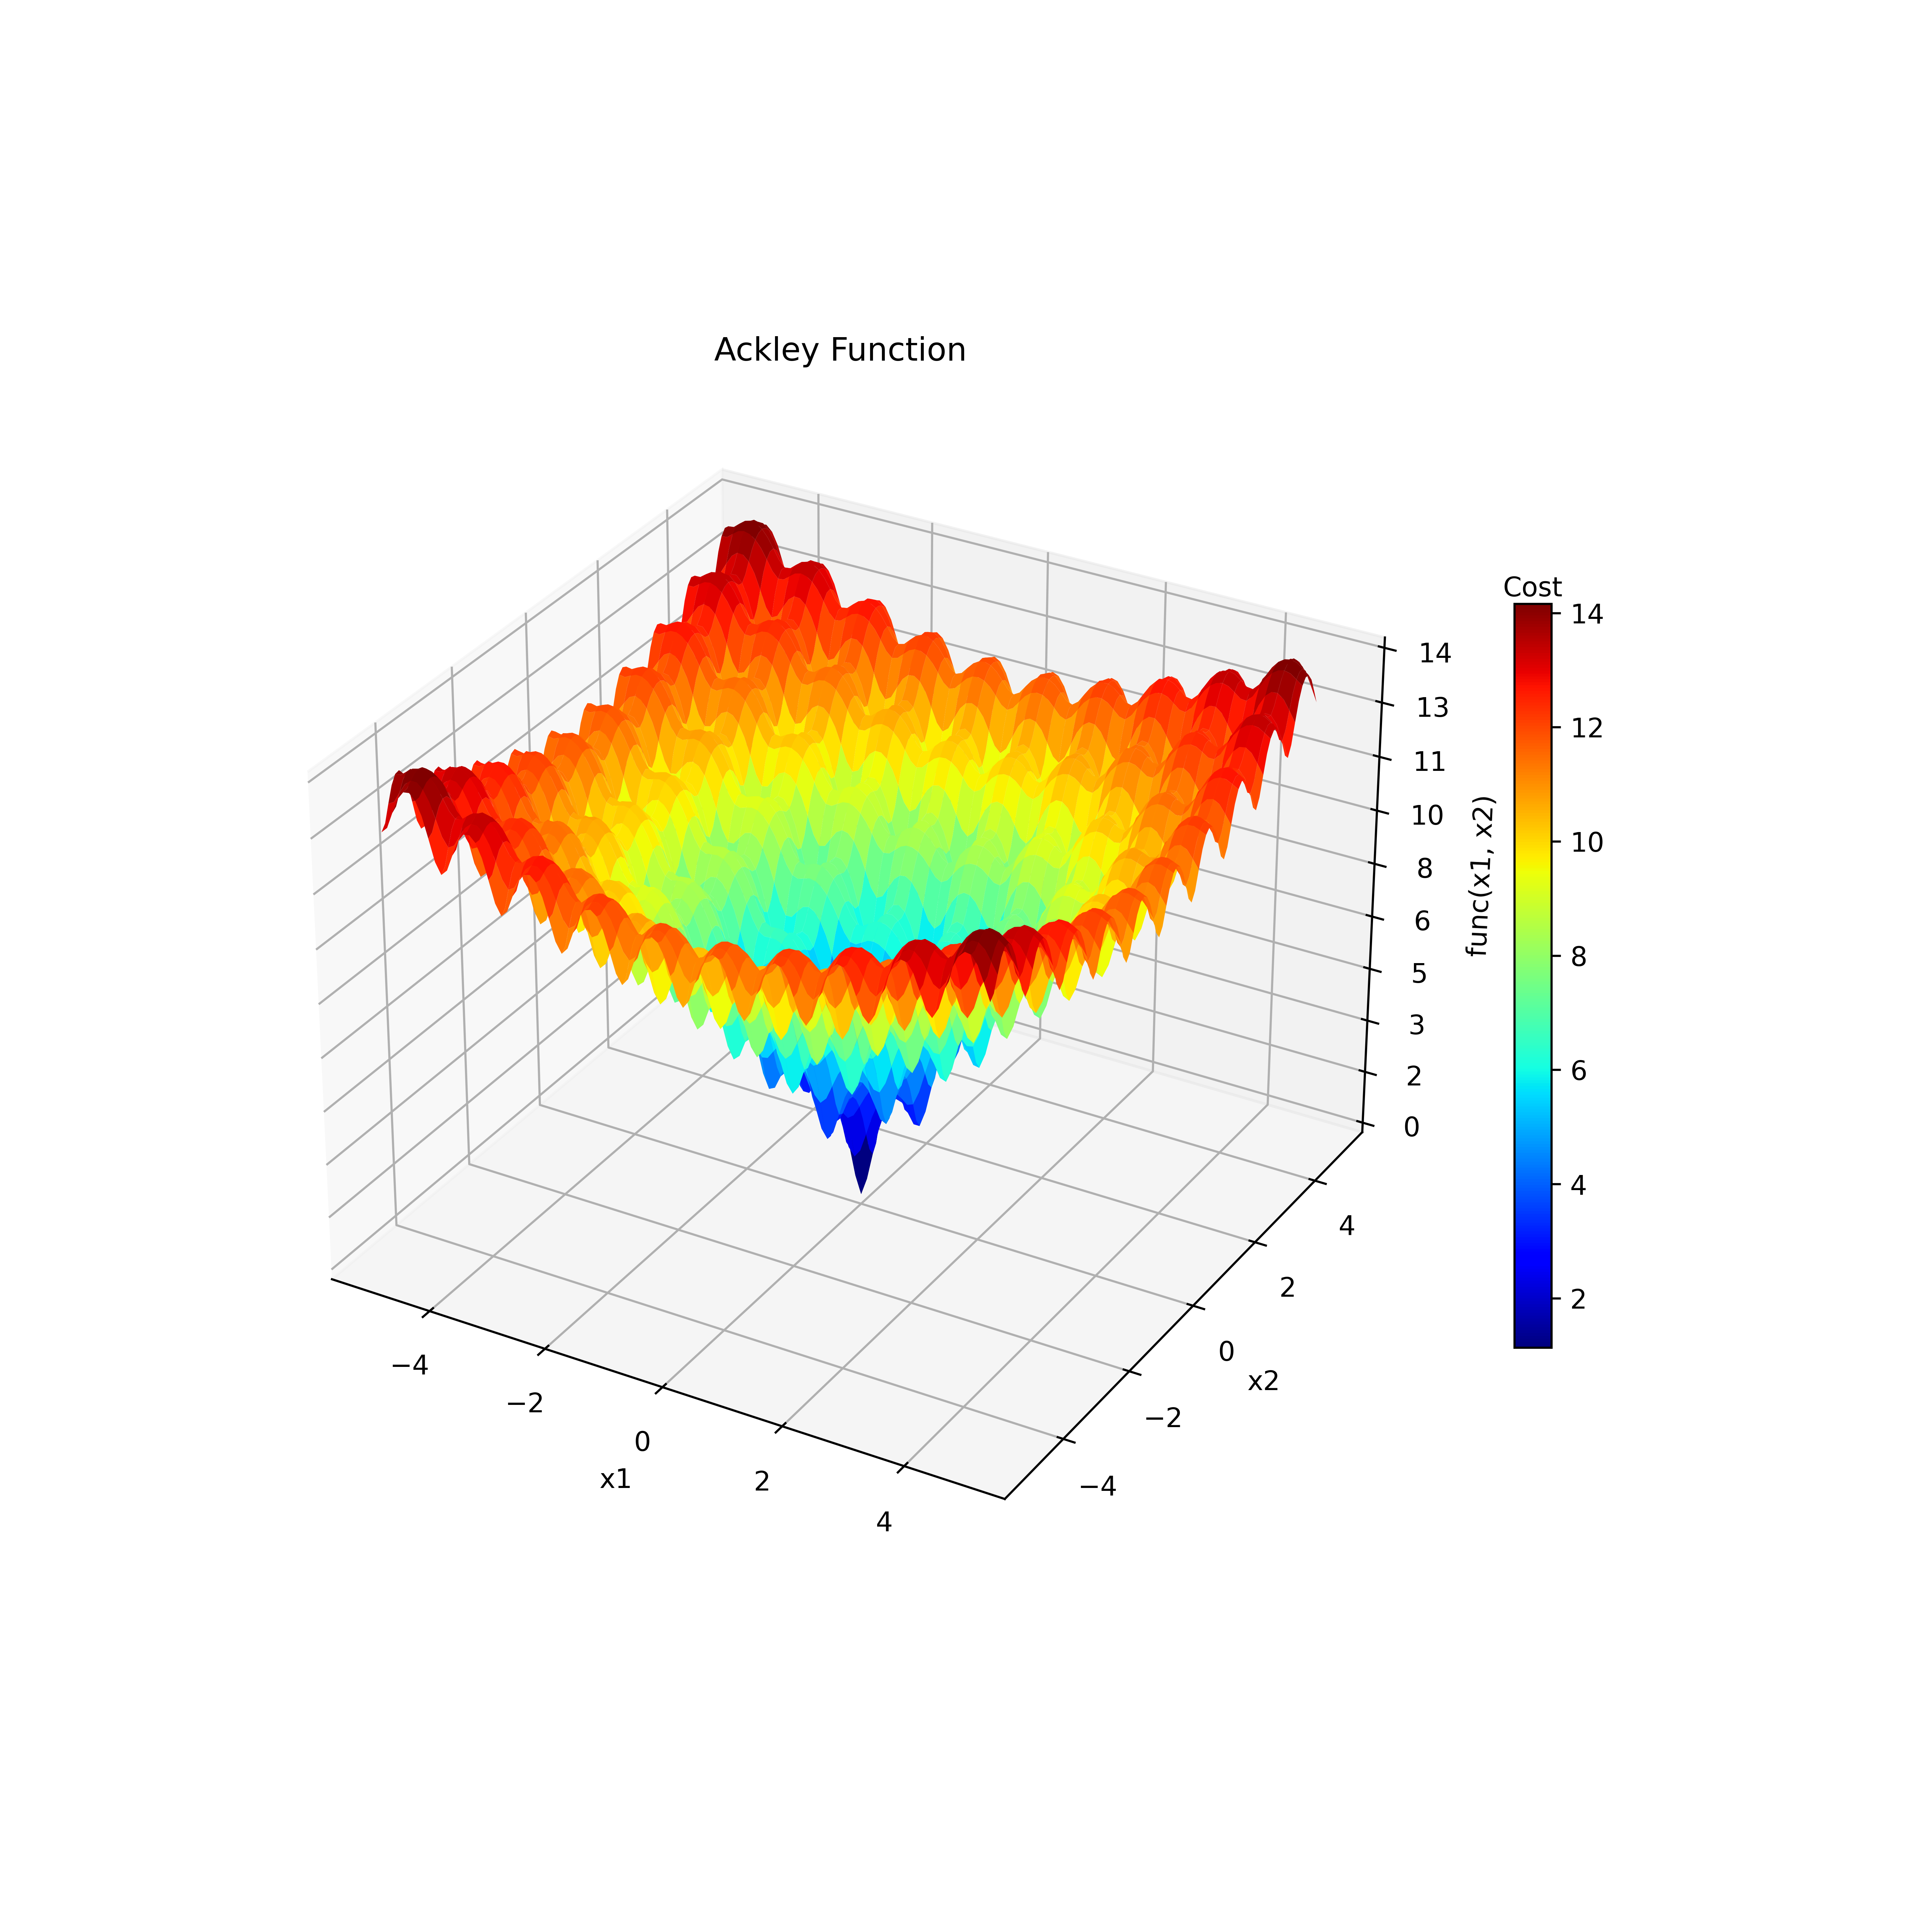
\includegraphics[width=0.8\paperwidth]{Fig/ackley.png}
%	\caption{Ackley function.}
%	\label{fig:ackley}
%\end{figure} 
%\begin{figure}	
%	\centering
%	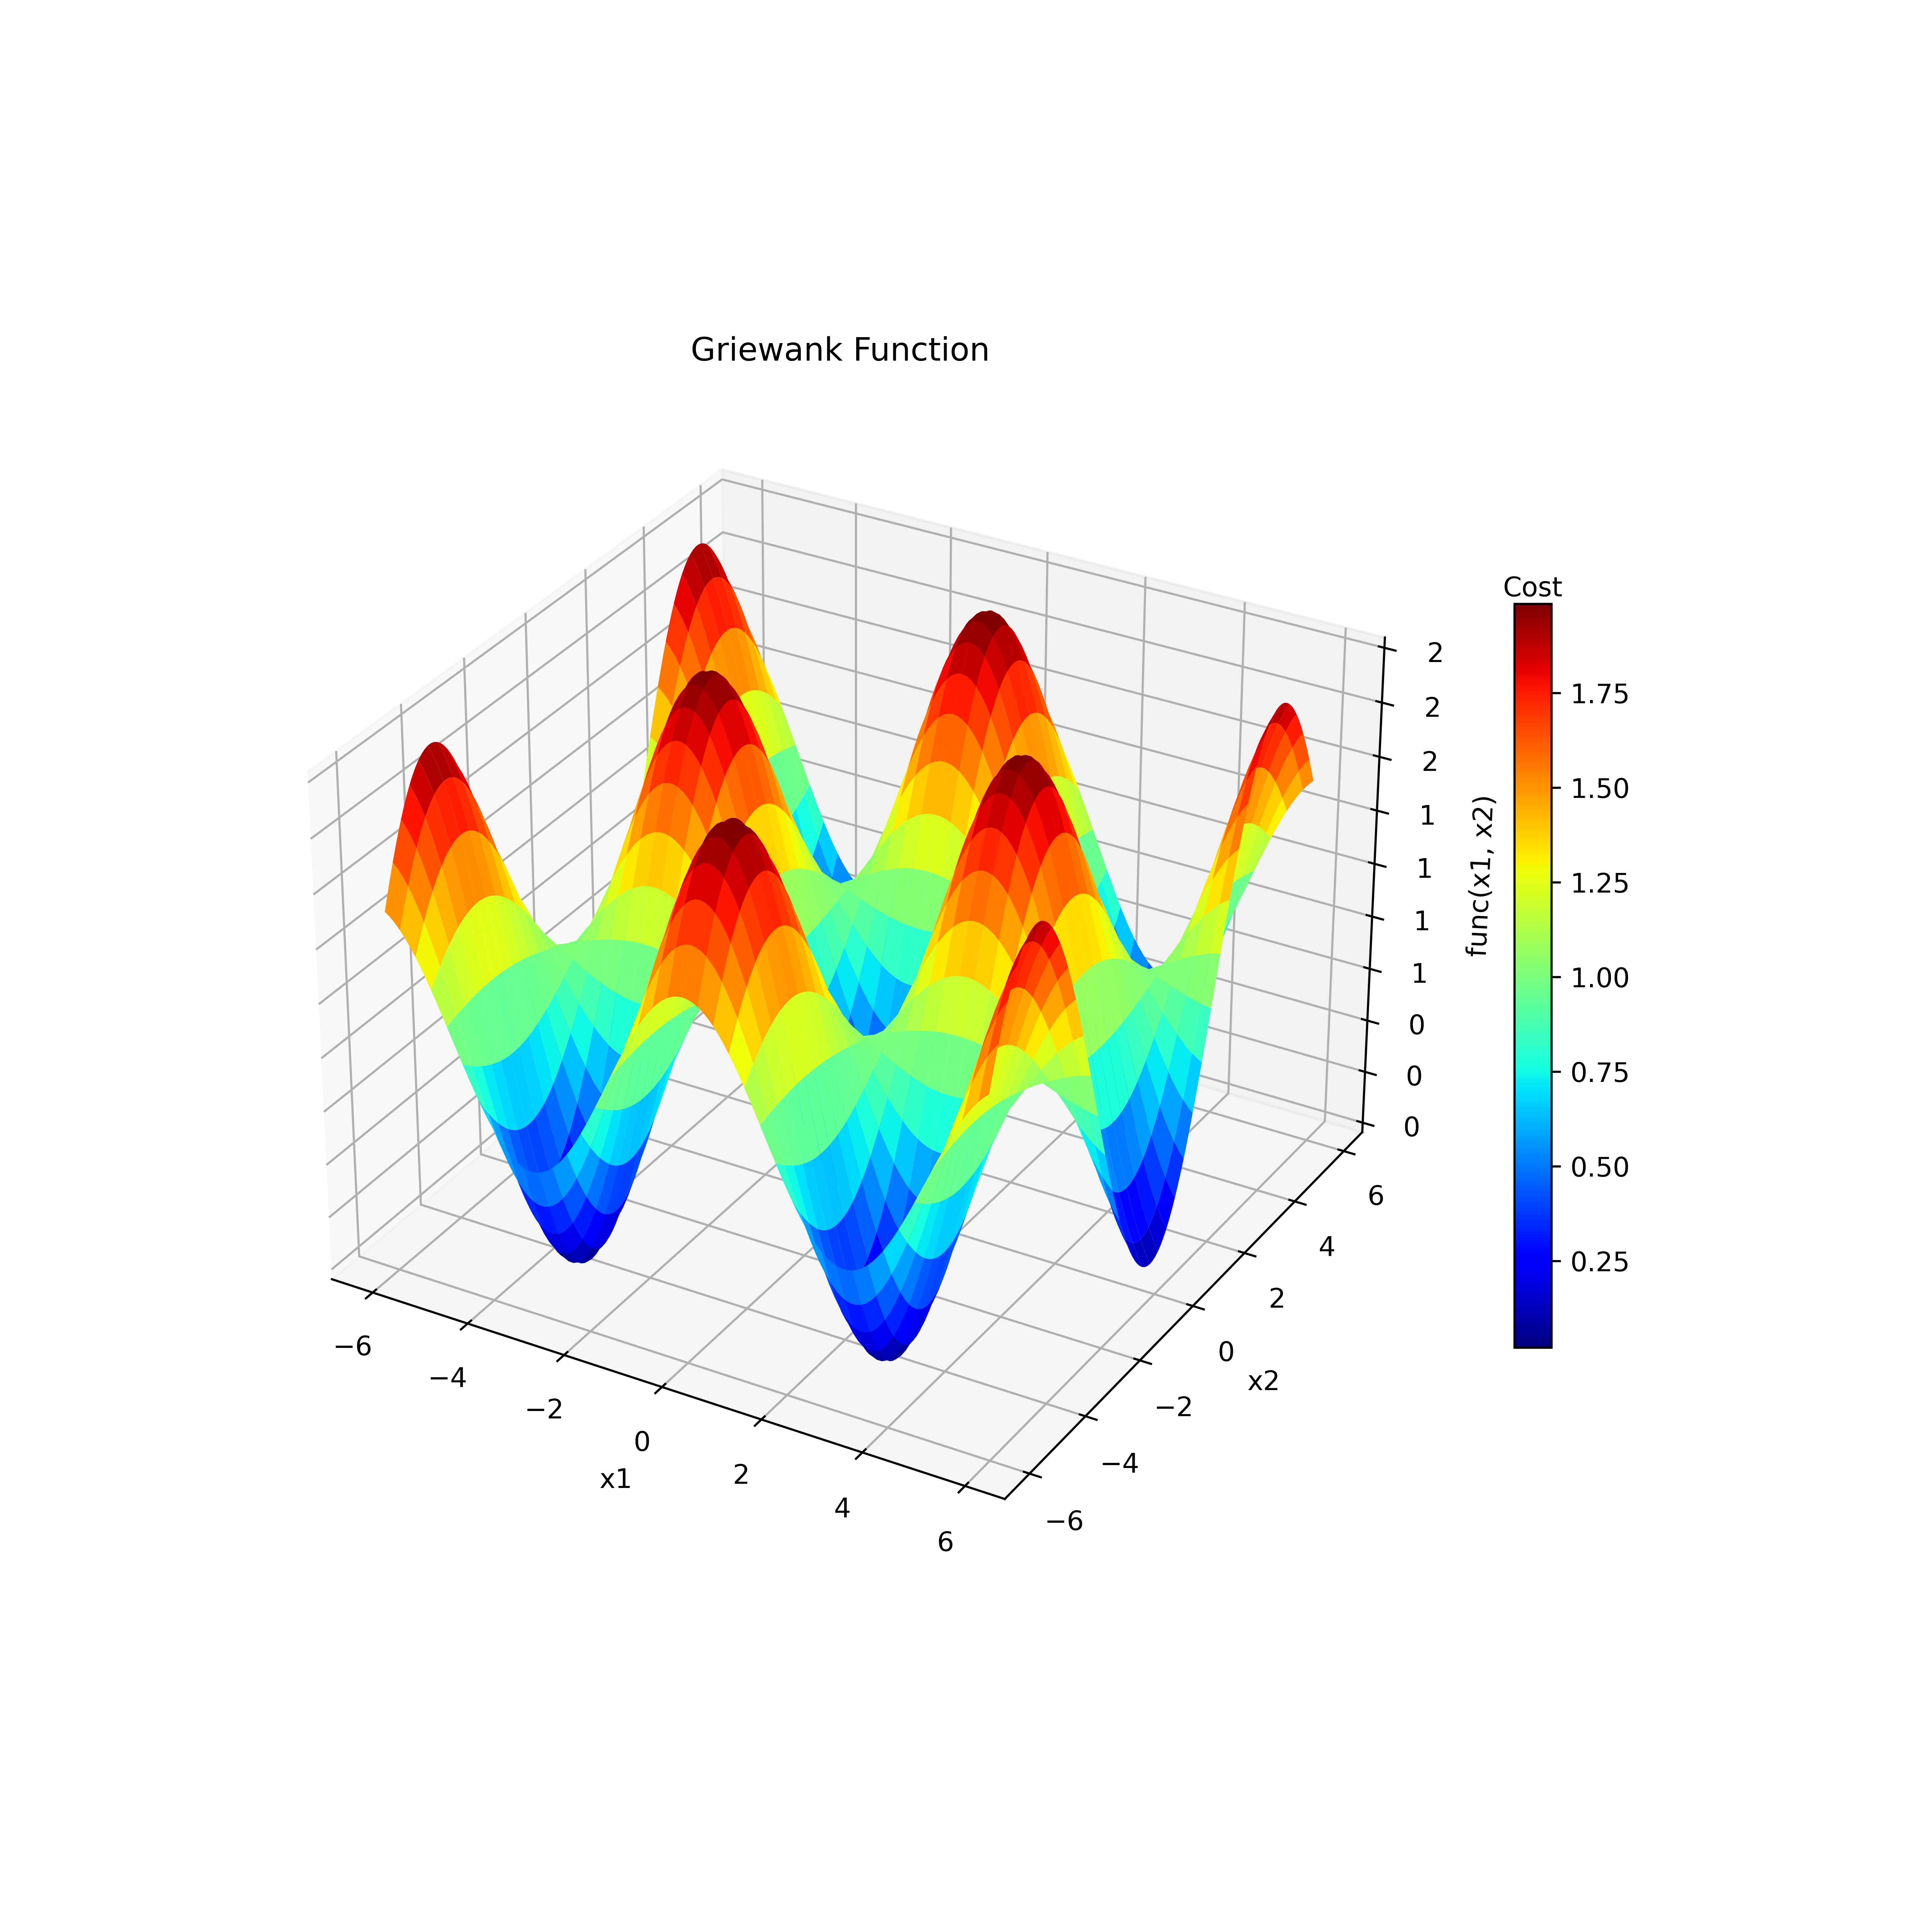
\includegraphics[width=0.8\paperwidth]{Fig/griewank.png}
%	\caption{Griewank function.}
%	\label{fig:griewank}
%\end{figure}
%\begin{figure}	
%	\centering
%	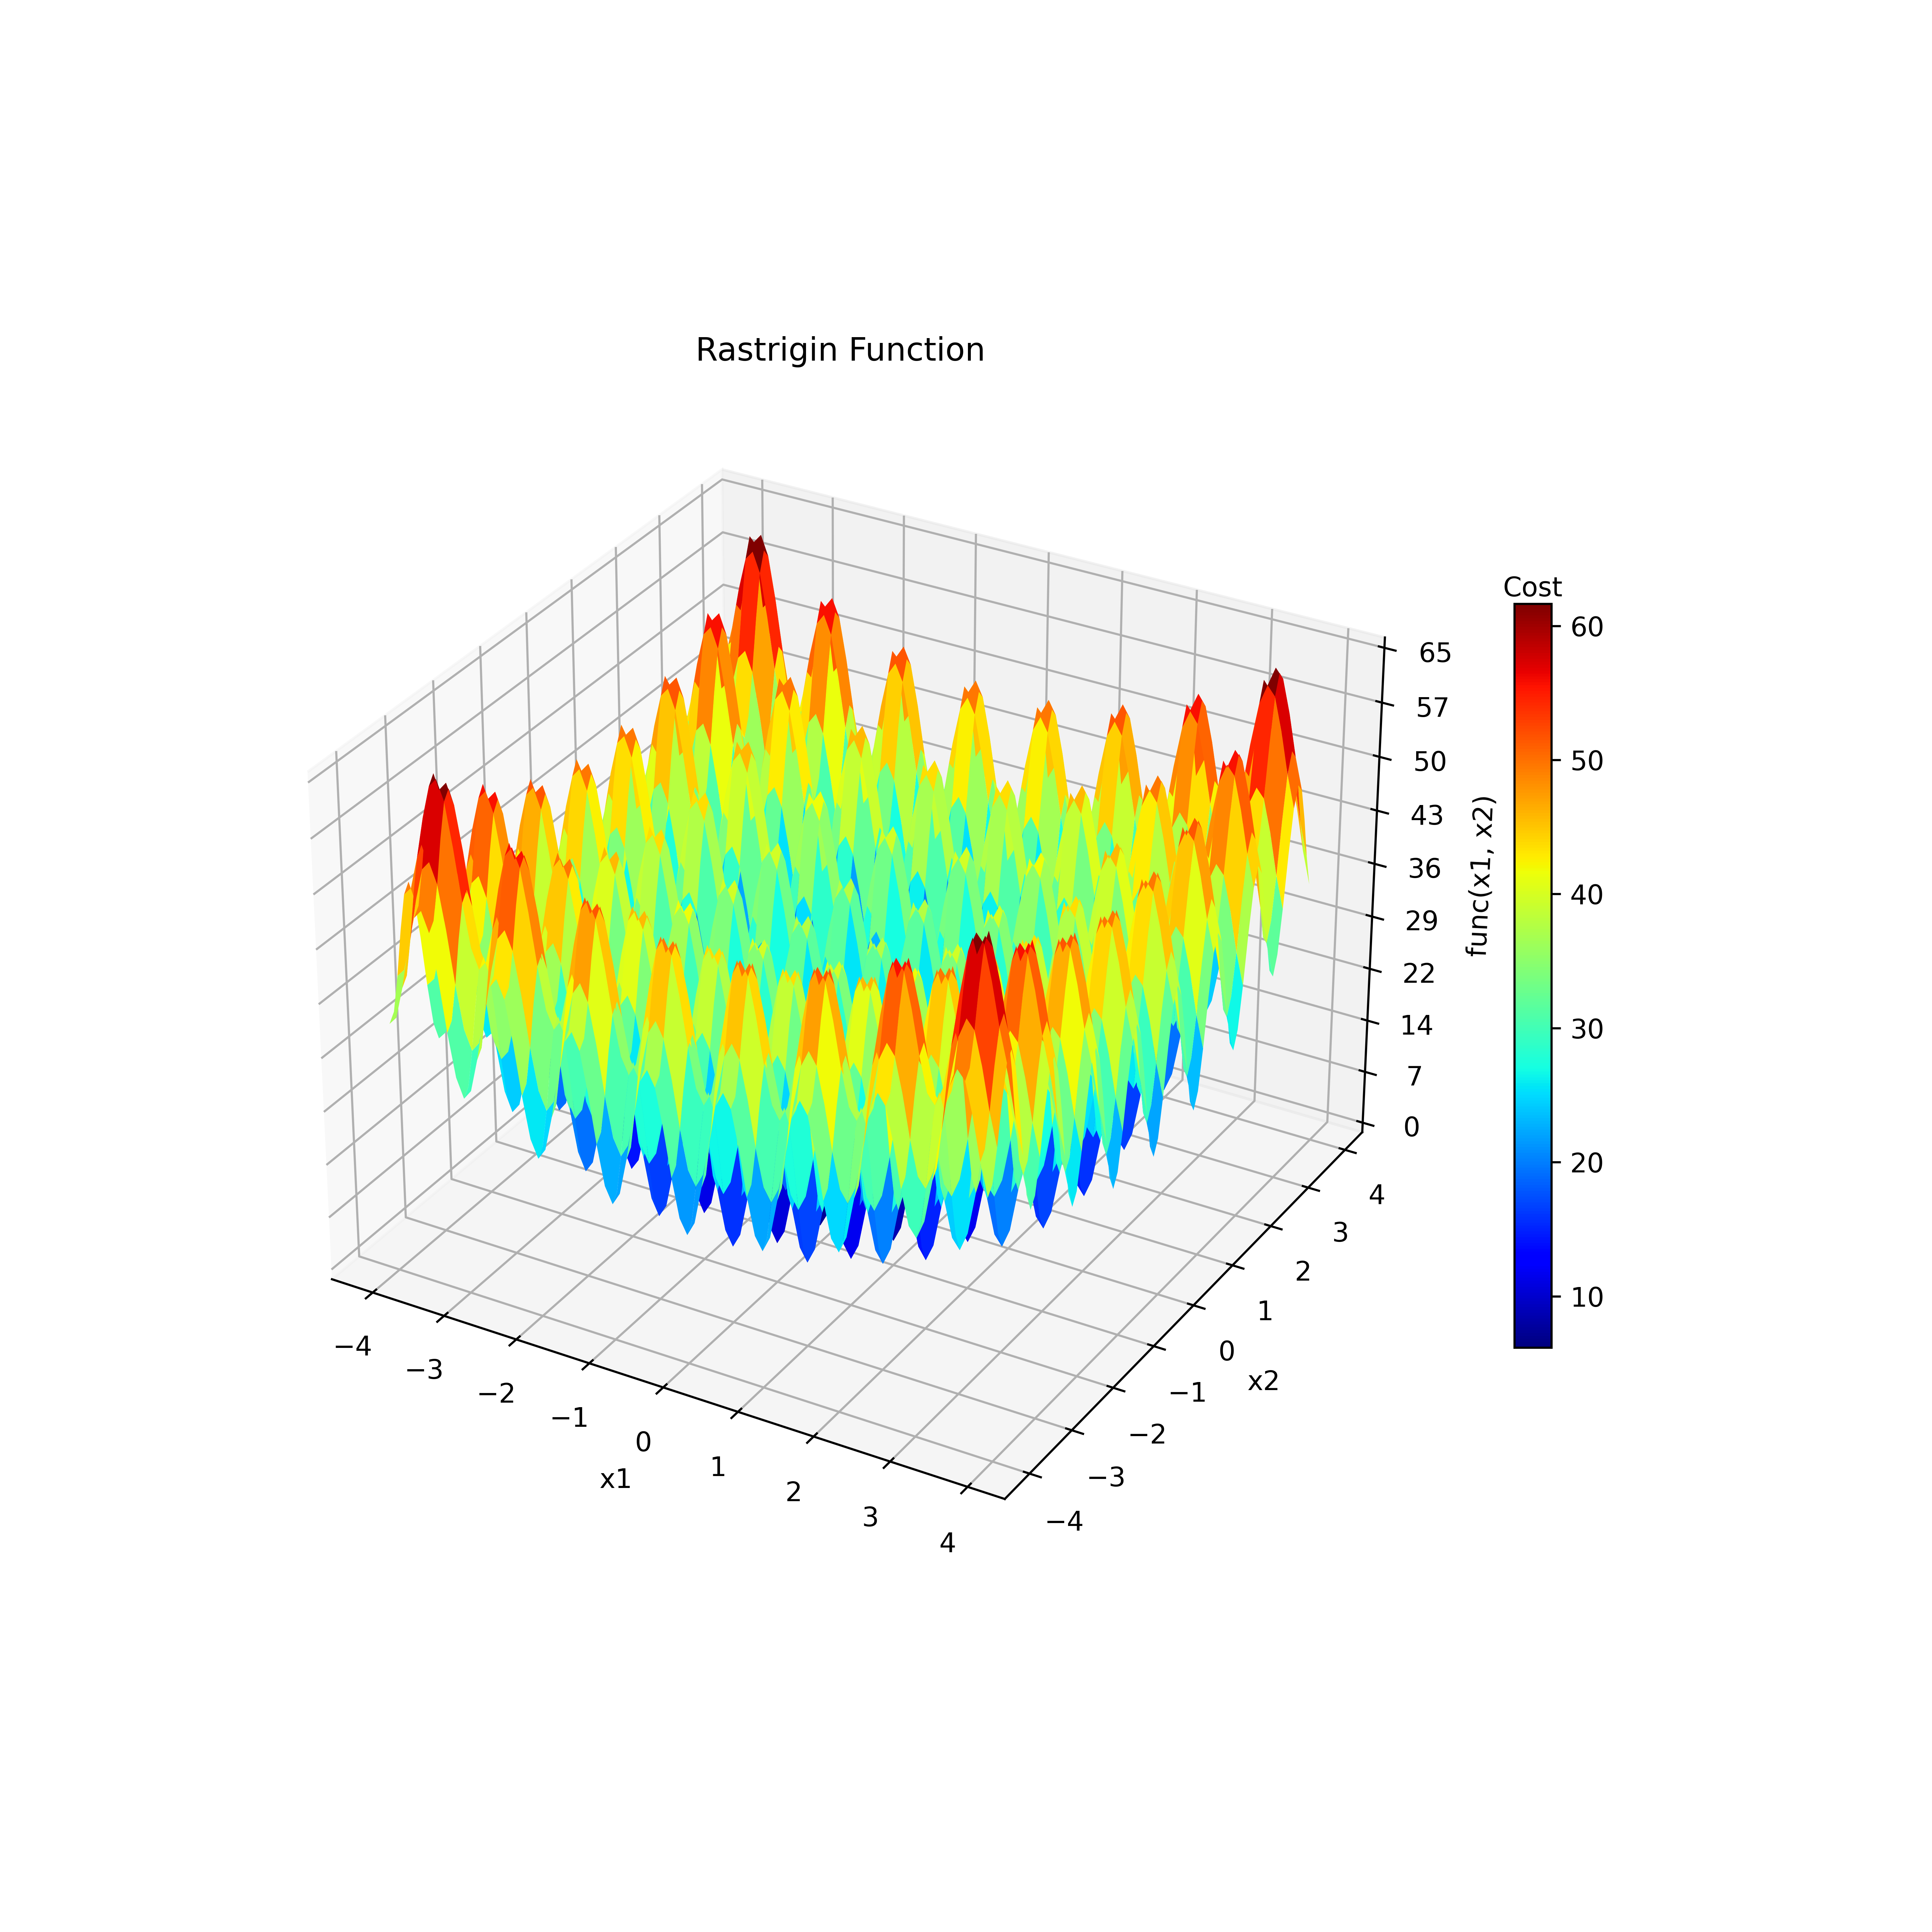
\includegraphics[width=0.8\paperwidth]{Fig/rastrigin.png}
%	\caption{Rastrigin function.}
%	\label{fig:rastrigin}
%\end{figure}
%\begin{figure}
%	\centering	
%	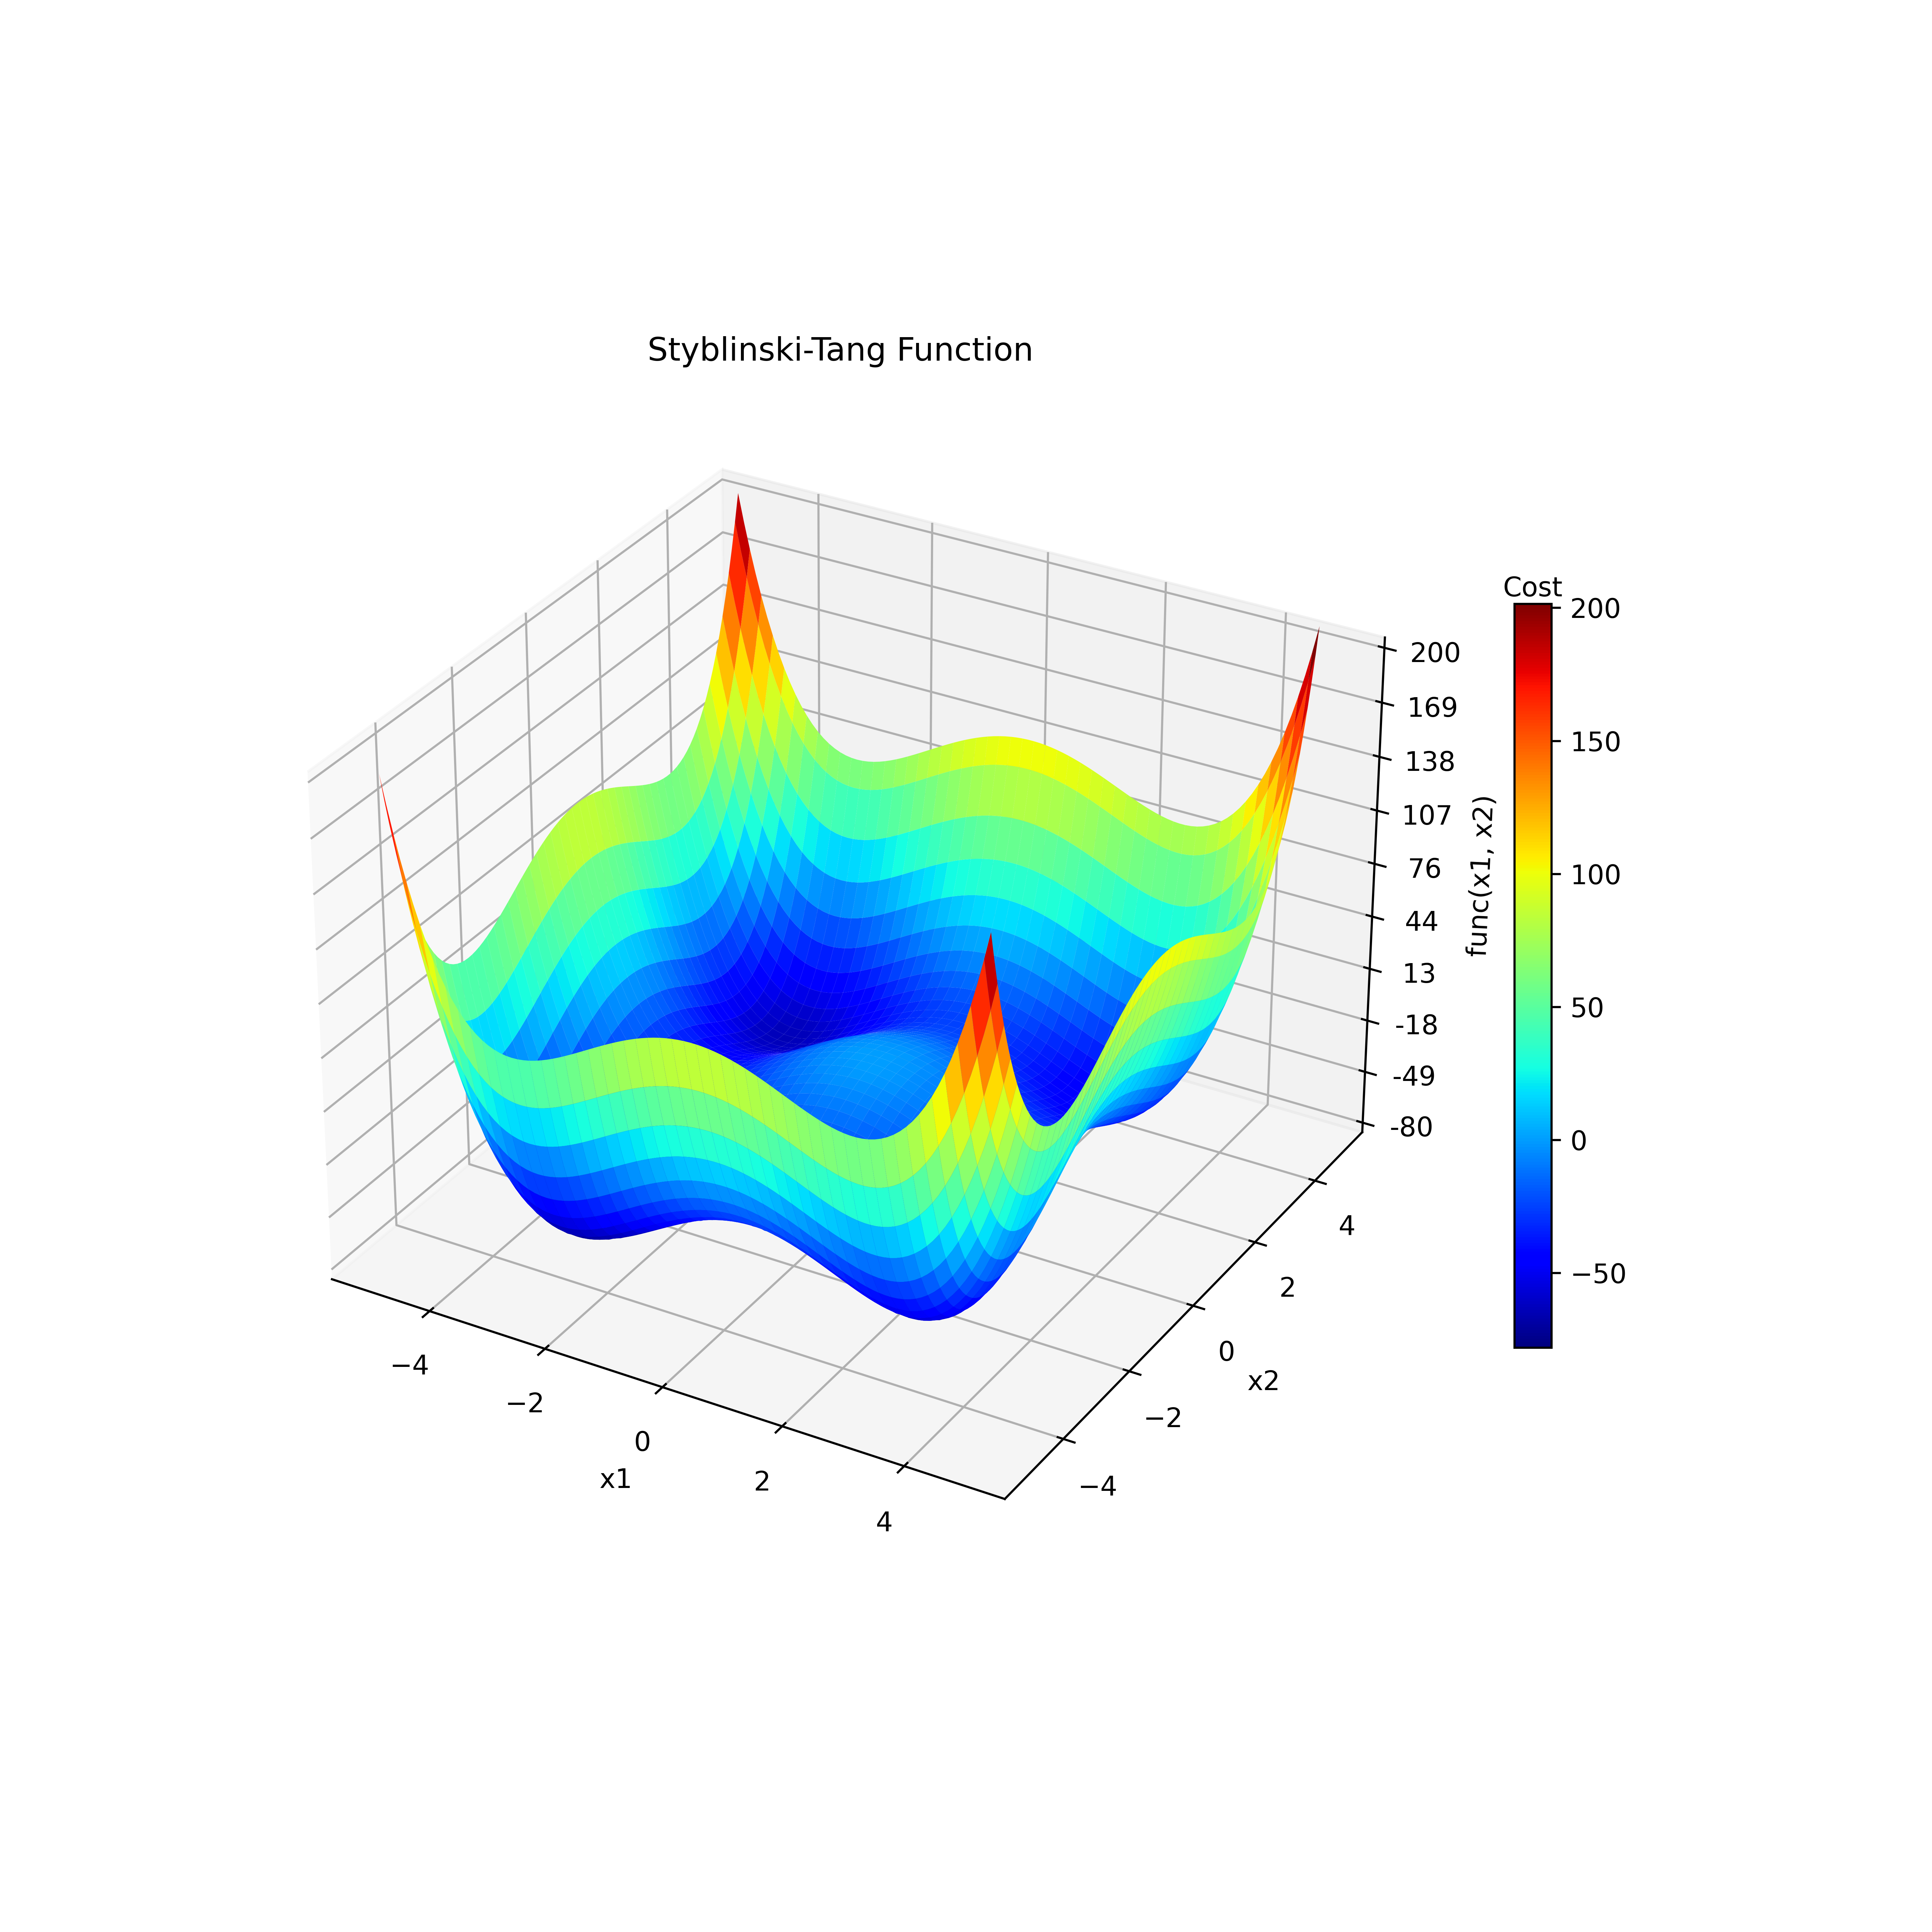
\includegraphics[width=0.8\paperwidth]{Fig/styblinski.png}
%	\caption{Styblinski-Tang function.}
%	\label{fig:styblinski}
%\end{figure}
%\begin{figure}	
%	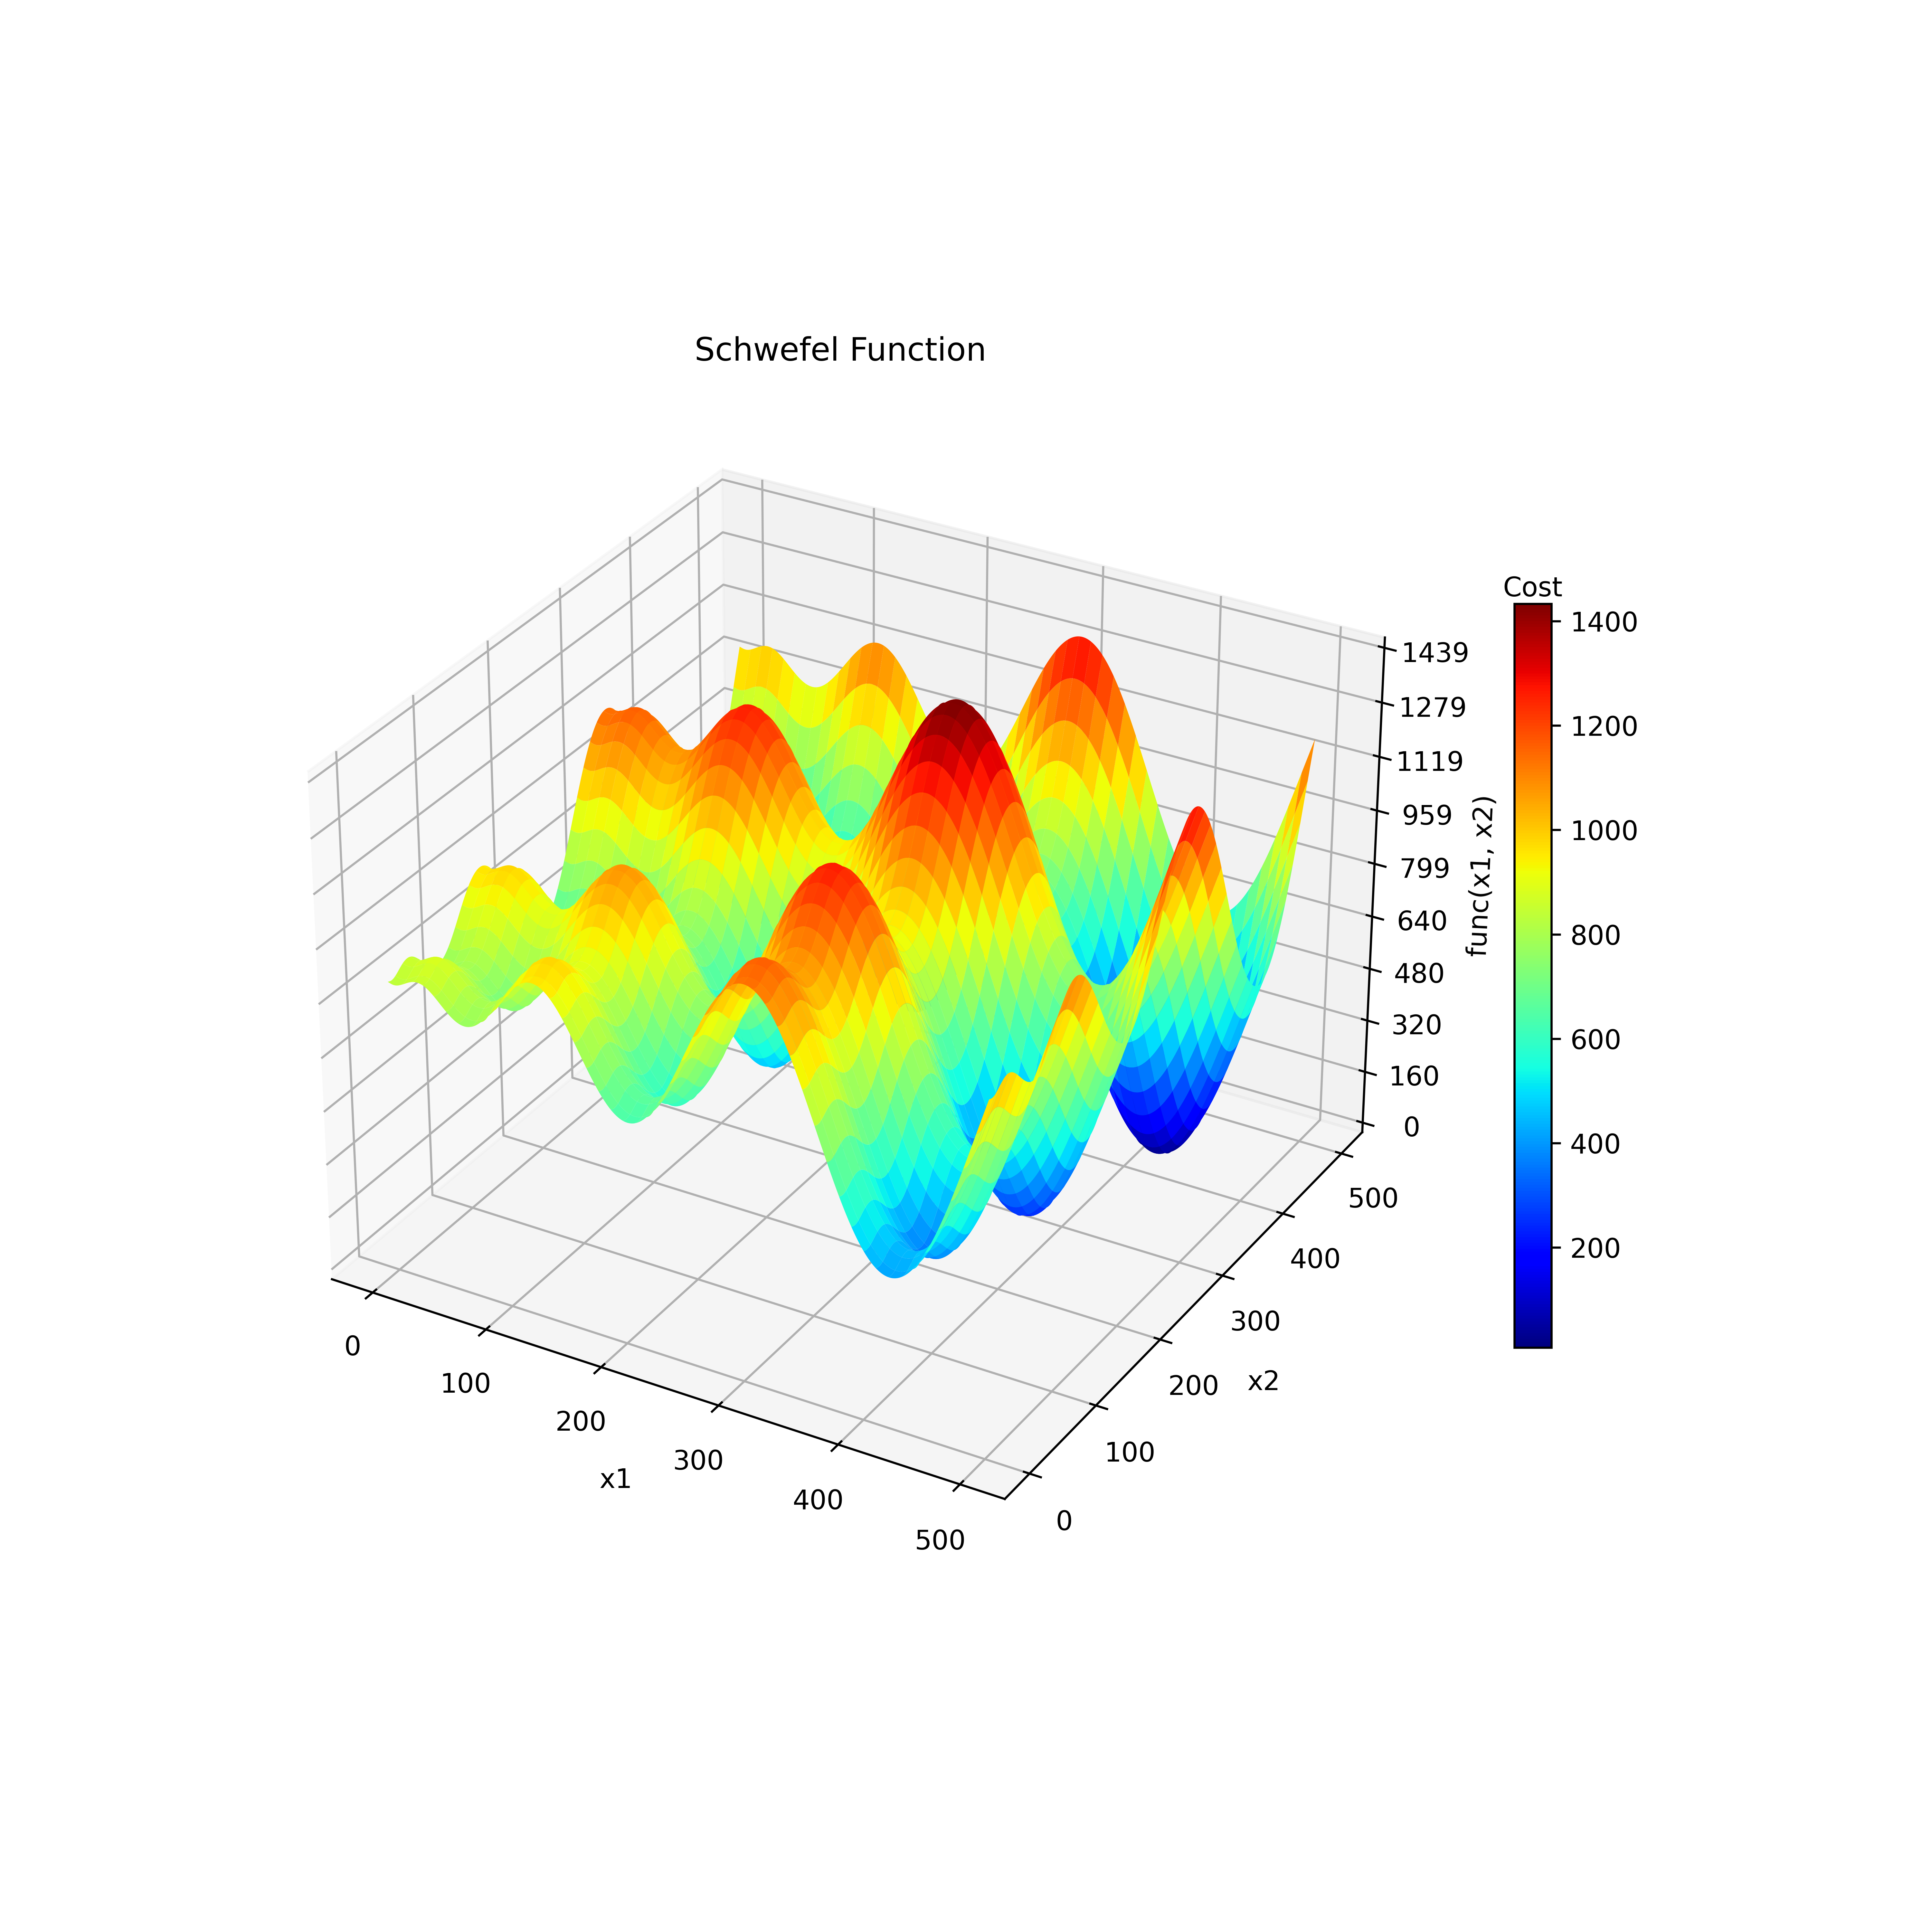
\includegraphics[width=0.8\paperwidth]{Fig/schwefel.png}
%	\caption{Schwefel function.}
%	\label{fig:schwefel}
%\end{figure}
%


%\verbatiminput{geophysics_paper.tex}

\append{The source of the bibliography}

%\verbatiminput{geophysics_reference.bib}

\newpage

\bibliographystyle{seg}  % style file is seg.bst
\bibliography{geophysics_reference}

\end{document}
